\documentclass[11pt]{article}
\usepackage[T1]{fontenc}
\usepackage{lmodern}
\usepackage[margin=1in]{geometry}
\usepackage{amsmath,amssymb,amsthm}
\usepackage{booktabs,longtable}
\usepackage[hidelinks]{hyperref}
\usepackage{url}

\usepackage{float}
\usepackage{tikz}
\usepackage{algorithm}
\usepackage[noend]{algpseudocode}

\newcommand{\NumImproved}{18}
\newcommand{\NumImprovedWord}{eighteen}
\newcommand{\NumImprovedWordCap}{Eighteen}
\newcommand{\NumOpen}{43}
\newcommand{\NumClosedNew}{0}
\newcommand{\NumUBImproved}{19}
\newcommand{\NumUBImprovedWord}{nineteen}
\newcommand{\ClosedList}{}
\newcommand{\MaxGain}{7}
\newcommand{\TotalGain}{58}
\newcommand{\Mmin}{13}\newcommand{\Mmax}{16}
\newcommand{\Nmin}{18}\newcommand{\Nmax}{23}
\newcommand{\NumPreprintDep}{7}


\title{\bfseries\boldmath Improved bounds and two exact values\\ for the Zarankiewicz numbers $z(m,n;3,3)$}
\author{JO\~AO AMARO}
\date{\today}

\begin{document}
\maketitle

\begin{abstract}
We improve the best known lower bounds for \NumImprovedWord{} Zarankiewicz
numbers $z(m,n;3,3)$, with $\Mmin\le m\le \Mmax$ and $\Nmin\le n\le \Nmax$,
by up to \MaxGain. The new matrices were found by a local search that
treats all cells together and passes each improvement to the neighbouring
cells. Combining an elementary deletion argument with two computer-assisted
methods, the elimination of column-degree profiles by exactly certified
linear programming and an exhaustive orderly generation, we improve
\NumUBImprovedWord{} upper bounds and determine \ClosedList. We summarize
the bounds from the recent literature in this range.
\end{abstract}

\section{Introduction}

The Zarankiewicz number $z(m,n;s,t)$ is the maximum number of ones in an
$m\times n$ $(0,1)$-matrix with no $s\times t$ all-ones submatrix
\cite{Zar51,KST54}. Equivalently, it is the maximum number of edges in a
subgraph of $K_{m,n}$ with no $K_{s,t}$ having its $s$ vertices in the part
of size $m$; the matrix is the biadjacency matrix of the graph. We study
$s=t=3$ and write $z(m,n)=z(m,n;3,3)=z(n,m)$.

Small values were tabulated by Guy~\cite{Guy69}, Collins et
al.~\cite{CRWR16} and Tan~\cite{Tan22}. General upper bounds include those
of Roman~\cite{Rom75} and of Davies, Gill and Horsley~\cite{DGH26}.
Recently, Bhan et al.~\cite{BNRL26} used an LLM-guided evolutionary search
to find lower bounds for $8\le m\le 16$, $16\le n\le 23$. They determined
three values exactly and left \NumOpen{} cells open. Some of these were
later settled or improved by Afrasyab~\cite{Afr26}, Hou~\cite{Hou26} and
Saurabh~\cite{Sau26}, and in a public repository of computer-certified
results~\cite{Fie26}.

This note builds on these works and makes three contributions.
\begin{itemize}
  \item \emph{Lower bounds} (Section~\ref{sec:lower}). We improve the lower
    bound in \NumImprovedWord{} cells, by up to \MaxGain, with explicit
    matrices found by a local search.
  \item \emph{Upper bounds} (Section~\ref{sec:upper}). The density lemma of
    Collins et al.~\cite{CRWR16}, applied to known exact values, together
    with profile elimination by exact linear programming (extending
    \cite{Afr26}) and an orderly generation, improves \NumUBImproved{}
    upper bounds and determines \ClosedList. The deletion argument had
    already been used in~\cite{Fie26} to settle three other cells.
  \item \emph{Summary} (Section~\ref{sec:known}). Table~\ref{tab:summary}
    and Figure~\ref{fig:heatmap} give the bounds for all \NumOpen{} cells
    with their sources. Some cells listed as open in~\cite{BNRL26} were
    already settled in~\cite{Tan22,CRWR16}.
\end{itemize}
The matrices, the verifier, the search code and the scripts that produce
the tables are available at
\url{https://github.com/joaoamaro70/zarankiewicz}.

\begin{figure}[t]
\centering
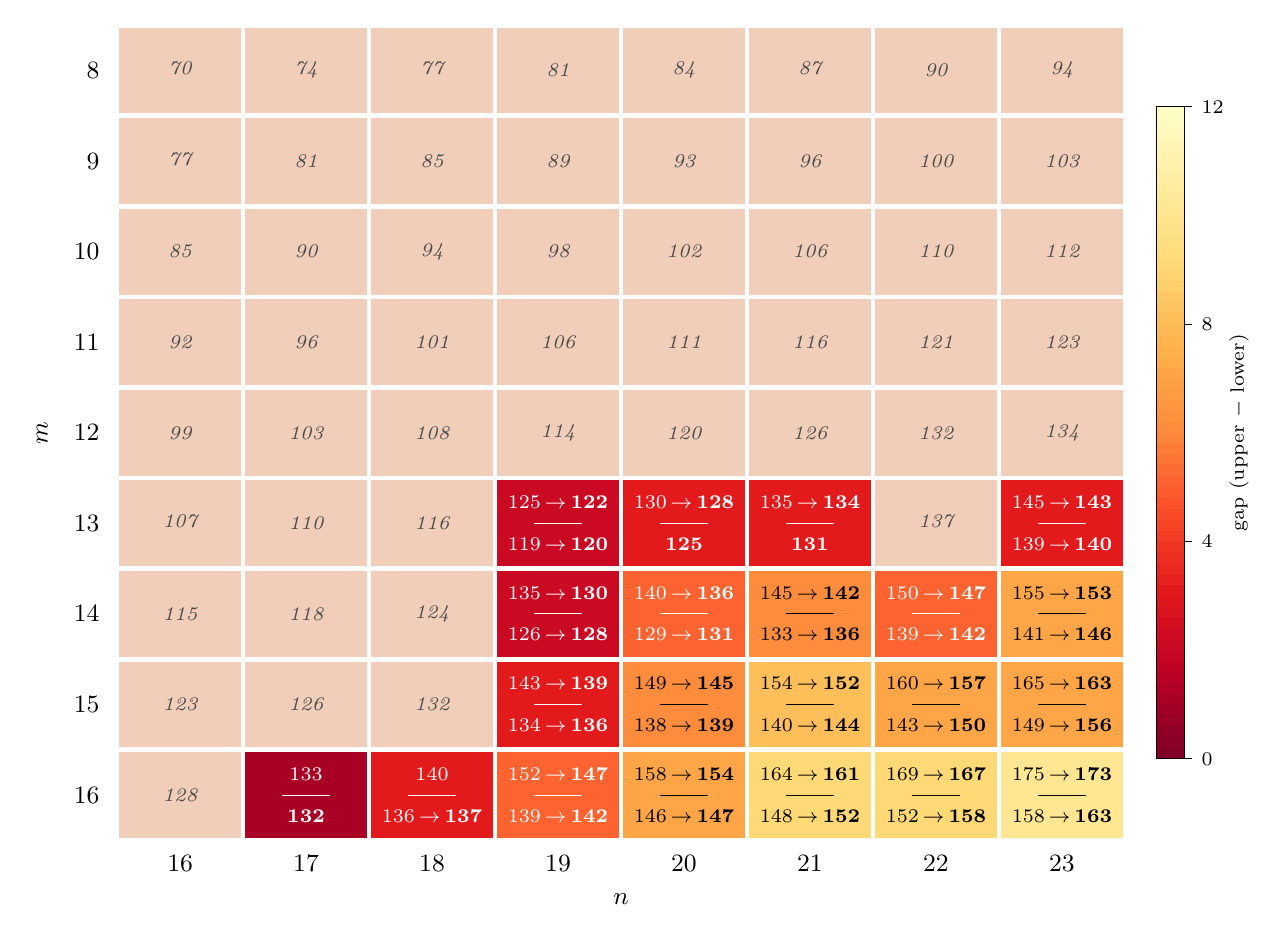
\begin{tikzpicture}[font=\scriptsize]
\node[anchor=east,font=\small] at (-0.1,9.775) {8};
\fill[fill={rgb,255:red,240;green,206;blue,186}] (0.030,9.230) rectangle (1.570,10.320);
\node[text=black!70] at (0.800,9.775) {\itshape 70};
\fill[fill={rgb,255:red,240;green,206;blue,186}] (1.630,9.230) rectangle (3.170,10.320);
\node[text=black!70] at (2.400,9.775) {\itshape 74};
\fill[fill={rgb,255:red,240;green,206;blue,186}] (3.230,9.230) rectangle (4.770,10.320);
\node[text=black!70] at (4.000,9.775) {\itshape 77};
\fill[fill={rgb,255:red,240;green,206;blue,186}] (4.830,9.230) rectangle (6.370,10.320);
\node[text=black!70] at (5.600,9.775) {\itshape 81};
\fill[fill={rgb,255:red,240;green,206;blue,186}] (6.430,9.230) rectangle (7.970,10.320);
\node[text=black!70] at (7.200,9.775) {\itshape 84};
\fill[fill={rgb,255:red,240;green,206;blue,186}] (8.030,9.230) rectangle (9.570,10.320);
\node[text=black!70] at (8.800,9.775) {\itshape 87};
\fill[fill={rgb,255:red,240;green,206;blue,186}] (9.630,9.230) rectangle (11.170,10.320);
\node[text=black!70] at (10.400,9.775) {\itshape 90};
\fill[fill={rgb,255:red,240;green,206;blue,186}] (11.230,9.230) rectangle (12.770,10.320);
\node[text=black!70] at (12.000,9.775) {\itshape 94};
\node[anchor=east,font=\small] at (-0.1,8.625) {9};
\fill[fill={rgb,255:red,240;green,206;blue,186}] (0.030,8.080) rectangle (1.570,9.170);
\node[text=black!70] at (0.800,8.625) {\itshape 77};
\fill[fill={rgb,255:red,240;green,206;blue,186}] (1.630,8.080) rectangle (3.170,9.170);
\node[text=black!70] at (2.400,8.625) {\itshape 81};
\fill[fill={rgb,255:red,240;green,206;blue,186}] (3.230,8.080) rectangle (4.770,9.170);
\node[text=black!70] at (4.000,8.625) {\itshape 85};
\fill[fill={rgb,255:red,240;green,206;blue,186}] (4.830,8.080) rectangle (6.370,9.170);
\node[text=black!70] at (5.600,8.625) {\itshape 89};
\fill[fill={rgb,255:red,240;green,206;blue,186}] (6.430,8.080) rectangle (7.970,9.170);
\node[text=black!70] at (7.200,8.625) {\itshape 93};
\fill[fill={rgb,255:red,240;green,206;blue,186}] (8.030,8.080) rectangle (9.570,9.170);
\node[text=black!70] at (8.800,8.625) {\itshape 96};
\fill[fill={rgb,255:red,240;green,206;blue,186}] (9.630,8.080) rectangle (11.170,9.170);
\node[text=black!70] at (10.400,8.625) {\itshape 100};
\fill[fill={rgb,255:red,240;green,206;blue,186}] (11.230,8.080) rectangle (12.770,9.170);
\node[text=black!70] at (12.000,8.625) {\itshape 103};
\node[anchor=east,font=\small] at (-0.1,7.475) {10};
\fill[fill={rgb,255:red,240;green,206;blue,186}] (0.030,6.930) rectangle (1.570,8.020);
\node[text=black!70] at (0.800,7.475) {\itshape 85};
\fill[fill={rgb,255:red,240;green,206;blue,186}] (1.630,6.930) rectangle (3.170,8.020);
\node[text=black!70] at (2.400,7.475) {\itshape 90};
\fill[fill={rgb,255:red,240;green,206;blue,186}] (3.230,6.930) rectangle (4.770,8.020);
\node[text=black!70] at (4.000,7.475) {\itshape 94};
\fill[fill={rgb,255:red,240;green,206;blue,186}] (4.830,6.930) rectangle (6.370,8.020);
\node[text=black!70] at (5.600,7.475) {\itshape 98};
\fill[fill={rgb,255:red,240;green,206;blue,186}] (6.430,6.930) rectangle (7.970,8.020);
\node[text=black!70] at (7.200,7.475) {\itshape 102};
\fill[fill={rgb,255:red,240;green,206;blue,186}] (8.030,6.930) rectangle (9.570,8.020);
\node[text=black!70] at (8.800,7.475) {\itshape 106};
\fill[fill={rgb,255:red,240;green,206;blue,186}] (9.630,6.930) rectangle (11.170,8.020);
\node[text=black!70] at (10.400,7.475) {\itshape 110};
\fill[fill={rgb,255:red,240;green,206;blue,186}] (11.230,6.930) rectangle (12.770,8.020);
\node[text=black!70] at (12.000,7.475) {\itshape 112};
\node[anchor=east,font=\small] at (-0.1,6.325) {11};
\fill[fill={rgb,255:red,240;green,206;blue,186}] (0.030,5.780) rectangle (1.570,6.870);
\node[text=black!70] at (0.800,6.325) {\itshape 92};
\fill[fill={rgb,255:red,240;green,206;blue,186}] (1.630,5.780) rectangle (3.170,6.870);
\node[text=black!70] at (2.400,6.325) {\itshape 96};
\fill[fill={rgb,255:red,240;green,206;blue,186}] (3.230,5.780) rectangle (4.770,6.870);
\node[text=black!70] at (4.000,6.325) {\itshape 101};
\fill[fill={rgb,255:red,240;green,206;blue,186}] (4.830,5.780) rectangle (6.370,6.870);
\node[text=black!70] at (5.600,6.325) {\itshape 106};
\fill[fill={rgb,255:red,240;green,206;blue,186}] (6.430,5.780) rectangle (7.970,6.870);
\node[text=black!70] at (7.200,6.325) {\itshape 111};
\fill[fill={rgb,255:red,240;green,206;blue,186}] (8.030,5.780) rectangle (9.570,6.870);
\node[text=black!70] at (8.800,6.325) {\itshape 116};
\fill[fill={rgb,255:red,240;green,206;blue,186}] (9.630,5.780) rectangle (11.170,6.870);
\node[text=black!70] at (10.400,6.325) {\itshape 121};
\fill[fill={rgb,255:red,240;green,206;blue,186}] (11.230,5.780) rectangle (12.770,6.870);
\node[text=black!70] at (12.000,6.325) {\itshape 123};
\node[anchor=east,font=\small] at (-0.1,5.175) {12};
\fill[fill={rgb,255:red,240;green,206;blue,186}] (0.030,4.630) rectangle (1.570,5.720);
\node[text=black!70] at (0.800,5.175) {\itshape 99};
\fill[fill={rgb,255:red,240;green,206;blue,186}] (1.630,4.630) rectangle (3.170,5.720);
\node[text=black!70] at (2.400,5.175) {\itshape 103};
\fill[fill={rgb,255:red,240;green,206;blue,186}] (3.230,4.630) rectangle (4.770,5.720);
\node[text=black!70] at (4.000,5.175) {\itshape 108};
\fill[fill={rgb,255:red,240;green,206;blue,186}] (4.830,4.630) rectangle (6.370,5.720);
\node[text=black!70] at (5.600,5.175) {\itshape 114};
\fill[fill={rgb,255:red,240;green,206;blue,186}] (6.430,4.630) rectangle (7.970,5.720);
\node[text=black!70] at (7.200,5.175) {\itshape 120};
\fill[fill={rgb,255:red,240;green,206;blue,186}] (8.030,4.630) rectangle (9.570,5.720);
\node[text=black!70] at (8.800,5.175) {\itshape 126};
\fill[fill={rgb,255:red,240;green,206;blue,186}] (9.630,4.630) rectangle (11.170,5.720);
\node[text=black!70] at (10.400,5.175) {\itshape 132};
\fill[fill={rgb,255:red,240;green,206;blue,186}] (11.230,4.630) rectangle (12.770,5.720);
\node[text=black!70] at (12.000,5.175) {\itshape 134};
\node[anchor=east,font=\small] at (-0.1,4.025) {13};
\fill[fill={rgb,255:red,240;green,206;blue,186}] (0.030,3.480) rectangle (1.570,4.570);
\node[text=black!70] at (0.800,4.025) {\itshape 107};
\fill[fill={rgb,255:red,240;green,206;blue,186}] (1.630,3.480) rectangle (3.170,4.570);
\node[text=black!70] at (2.400,4.025) {\itshape 110};
\fill[fill={rgb,255:red,240;green,206;blue,186}] (3.230,3.480) rectangle (4.770,4.570);
\node[text=black!70] at (4.000,4.025) {\itshape 116};
\fill[fill={rgb,255:red,202;green,9;blue,35}] (4.830,3.480) rectangle (6.370,4.570);
\node[text=white] at (5.600,4.289) {125$\,\to\,$\textbf{122}};
\draw[white,line width=0.3pt] (5.300,4.025) -- (5.900,4.025);
\node[text=white] at (5.600,3.760) {119$\,\to\,$\textbf{120}};
\fill[fill={rgb,255:red,227;green,26;blue,28}] (6.430,3.480) rectangle (7.970,4.570);
\node[text=white] at (7.200,4.289) {130$\,\to\,$\textbf{128}};
\draw[white,line width=0.3pt] (6.900,4.025) -- (7.500,4.025);
\node[text=white] at (7.200,3.760) {\textbf{125}};
\fill[fill={rgb,255:red,227;green,26;blue,28}] (8.030,3.480) rectangle (9.570,4.570);
\node[text=white] at (8.800,4.289) {135$\,\to\,$\textbf{134}};
\draw[white,line width=0.3pt] (8.500,4.025) -- (9.100,4.025);
\node[text=white] at (8.800,3.760) {\textbf{131}};
\fill[fill={rgb,255:red,240;green,206;blue,186}] (9.630,3.480) rectangle (11.170,4.570);
\node[text=black!70] at (10.400,4.025) {\itshape 137};
\fill[fill={rgb,255:red,227;green,26;blue,28}] (11.230,3.480) rectangle (12.770,4.570);
\node[text=white] at (12.000,4.289) {145$\,\to\,$\textbf{143}};
\draw[white,line width=0.3pt] (11.700,4.025) -- (12.300,4.025);
\node[text=white] at (12.000,3.760) {139$\,\to\,$\textbf{140}};
\node[anchor=east,font=\small] at (-0.1,2.875) {14};
\fill[fill={rgb,255:red,240;green,206;blue,186}] (0.030,2.330) rectangle (1.570,3.420);
\node[text=black!70] at (0.800,2.875) {\itshape 115};
\fill[fill={rgb,255:red,240;green,206;blue,186}] (1.630,2.330) rectangle (3.170,3.420);
\node[text=black!70] at (2.400,2.875) {\itshape 118};
\fill[fill={rgb,255:red,240;green,206;blue,186}] (3.230,2.330) rectangle (4.770,3.420);
\node[text=black!70] at (4.000,2.875) {\itshape 124};
\fill[fill={rgb,255:red,202;green,9;blue,35}] (4.830,2.330) rectangle (6.370,3.420);
\node[text=white] at (5.600,3.139) {135$\,\to\,$\textbf{130}};
\draw[white,line width=0.3pt] (5.300,2.875) -- (5.900,2.875);
\node[text=white] at (5.600,2.611) {126$\,\to\,$\textbf{128}};
\fill[fill={rgb,255:red,252;green,99;blue,48}] (6.430,2.330) rectangle (7.970,3.420);
\node[text=white] at (7.200,3.139) {140$\,\to\,$\textbf{136}};
\draw[white,line width=0.3pt] (6.900,2.875) -- (7.500,2.875);
\node[text=white] at (7.200,2.611) {129$\,\to\,$\textbf{131}};
\fill[fill={rgb,255:red,253;green,141;blue,60}] (8.030,2.330) rectangle (9.570,3.420);
\node[text=black] at (8.800,3.139) {145$\,\to\,$\textbf{142}};
\draw[black,line width=0.3pt] (8.500,2.875) -- (9.100,2.875);
\node[text=black] at (8.800,2.611) {133$\,\to\,$\textbf{136}};
\fill[fill={rgb,255:red,252;green,99;blue,48}] (9.630,2.330) rectangle (11.170,3.420);
\node[text=white] at (10.400,3.139) {150$\,\to\,$\textbf{147}};
\draw[white,line width=0.3pt] (10.100,2.875) -- (10.700,2.875);
\node[text=white] at (10.400,2.611) {139$\,\to\,$\textbf{142}};
\fill[fill={rgb,255:red,254;green,166;blue,71}] (11.230,2.330) rectangle (12.770,3.420);
\node[text=black] at (12.000,3.139) {155$\,\to\,$\textbf{153}};
\draw[black,line width=0.3pt] (11.700,2.875) -- (12.300,2.875);
\node[text=black] at (12.000,2.611) {141$\,\to\,$\textbf{146}};
\node[anchor=east,font=\small] at (-0.1,1.725) {15};
\fill[fill={rgb,255:red,240;green,206;blue,186}] (0.030,1.180) rectangle (1.570,2.270);
\node[text=black!70] at (0.800,1.725) {\itshape 123};
\fill[fill={rgb,255:red,240;green,206;blue,186}] (1.630,1.180) rectangle (3.170,2.270);
\node[text=black!70] at (2.400,1.725) {\itshape 126};
\fill[fill={rgb,255:red,240;green,206;blue,186}] (3.230,1.180) rectangle (4.770,2.270);
\node[text=black!70] at (4.000,1.725) {\itshape 132};
\fill[fill={rgb,255:red,227;green,26;blue,28}] (4.830,1.180) rectangle (6.370,2.270);
\node[text=white] at (5.600,1.989) {143$\,\to\,$\textbf{139}};
\draw[white,line width=0.3pt] (5.300,1.725) -- (5.900,1.725);
\node[text=white] at (5.600,1.460) {134$\,\to\,$\textbf{136}};
\fill[fill={rgb,255:red,253;green,141;blue,60}] (6.430,1.180) rectangle (7.970,2.270);
\node[text=black] at (7.200,1.989) {149$\,\to\,$\textbf{145}};
\draw[black,line width=0.3pt] (6.900,1.725) -- (7.500,1.725);
\node[text=black] at (7.200,1.460) {138$\,\to\,$\textbf{139}};
\fill[fill={rgb,255:red,254;green,191;blue,90}] (8.030,1.180) rectangle (9.570,2.270);
\node[text=black] at (8.800,1.989) {154$\,\to\,$\textbf{152}};
\draw[black,line width=0.3pt] (8.500,1.725) -- (9.100,1.725);
\node[text=black] at (8.800,1.460) {140$\,\to\,$\textbf{144}};
\fill[fill={rgb,255:red,254;green,166;blue,71}] (9.630,1.180) rectangle (11.170,2.270);
\node[text=black] at (10.400,1.989) {160$\,\to\,$\textbf{157}};
\draw[black,line width=0.3pt] (10.100,1.725) -- (10.700,1.725);
\node[text=black] at (10.400,1.460) {143$\,\to\,$\textbf{150}};
\fill[fill={rgb,255:red,254;green,166;blue,71}] (11.230,1.180) rectangle (12.770,2.270);
\node[text=black] at (12.000,1.989) {165$\,\to\,$\textbf{163}};
\draw[black,line width=0.3pt] (11.700,1.725) -- (12.300,1.725);
\node[text=black] at (12.000,1.460) {149$\,\to\,$\textbf{156}};
\node[anchor=east,font=\small] at (-0.1,0.575) {16};
\fill[fill={rgb,255:red,240;green,206;blue,186}] (0.030,0.030) rectangle (1.570,1.120);
\node[text=black!70] at (0.800,0.575) {\itshape 128};
\fill[fill={rgb,255:red,169;green,0;blue,38}] (1.630,0.030) rectangle (3.170,1.120);
\node[text=white] at (2.400,0.839) {133};
\draw[white,line width=0.3pt] (2.100,0.575) -- (2.700,0.575);
\node[text=white] at (2.400,0.310) {\textbf{132}};
\fill[fill={rgb,255:red,227;green,26;blue,28}] (3.230,0.030) rectangle (4.770,1.120);
\node[text=white] at (4.000,0.839) {140};
\draw[white,line width=0.3pt] (3.700,0.575) -- (4.300,0.575);
\node[text=white] at (4.000,0.310) {136$\,\to\,$\textbf{137}};
\fill[fill={rgb,255:red,252;green,99;blue,48}] (4.830,0.030) rectangle (6.370,1.120);
\node[text=white] at (5.600,0.839) {152$\,\to\,$\textbf{147}};
\draw[white,line width=0.3pt] (5.300,0.575) -- (5.900,0.575);
\node[text=white] at (5.600,0.310) {139$\,\to\,$\textbf{142}};
\fill[fill={rgb,255:red,254;green,166;blue,71}] (6.430,0.030) rectangle (7.970,1.120);
\node[text=black] at (7.200,0.839) {158$\,\to\,$\textbf{154}};
\draw[black,line width=0.3pt] (6.900,0.575) -- (7.500,0.575);
\node[text=black] at (7.200,0.310) {146$\,\to\,$\textbf{147}};
\fill[fill={rgb,255:red,254;green,217;blue,118}] (8.030,0.030) rectangle (9.570,1.120);
\node[text=black] at (8.800,0.839) {164$\,\to\,$\textbf{161}};
\draw[black,line width=0.3pt] (8.500,0.575) -- (9.100,0.575);
\node[text=black] at (8.800,0.310) {148$\,\to\,$\textbf{152}};
\fill[fill={rgb,255:red,254;green,217;blue,118}] (9.630,0.030) rectangle (11.170,1.120);
\node[text=black] at (10.400,0.839) {169$\,\to\,$\textbf{167}};
\draw[black,line width=0.3pt] (10.100,0.575) -- (10.700,0.575);
\node[text=black] at (10.400,0.310) {152$\,\to\,$\textbf{158}};
\fill[fill={rgb,255:red,255;green,230;blue,146}] (11.230,0.030) rectangle (12.770,1.120);
\node[text=black] at (12.000,0.839) {175$\,\to\,$\textbf{173}};
\draw[black,line width=0.3pt] (11.700,0.575) -- (12.300,0.575);
\node[text=black] at (12.000,0.310) {158$\,\to\,$\textbf{163}};
\node[font=\small] at (0.800,-0.3) {16};
\node[font=\small] at (2.400,-0.3) {17};
\node[font=\small] at (4.000,-0.3) {18};
\node[font=\small] at (5.600,-0.3) {19};
\node[font=\small] at (7.200,-0.3) {20};
\node[font=\small] at (8.800,-0.3) {21};
\node[font=\small] at (10.400,-0.3) {22};
\node[font=\small] at (12.000,-0.3) {23};
\node[font=\small] at (6.400,-0.75) {$n$};
\node[font=\small,rotate=90] at (-0.95,5.175) {$m$};
\fill[fill={rgb,255:red,128;green,0;blue,38}] (13.200000000000001,1.035) rectangle (13.55,1.175);
\fill[fill={rgb,255:red,136;green,0;blue,38}] (13.200000000000001,1.173) rectangle (13.55,1.313);
\fill[fill={rgb,255:red,144;green,0;blue,38}] (13.200000000000001,1.311) rectangle (13.55,1.451);
\fill[fill={rgb,255:red,152;green,0;blue,38}] (13.200000000000001,1.449) rectangle (13.55,1.589);
\fill[fill={rgb,255:red,161;green,0;blue,38}] (13.200000000000001,1.587) rectangle (13.55,1.727);
\fill[fill={rgb,255:red,169;green,0;blue,38}] (13.200000000000001,1.725) rectangle (13.55,1.865);
\fill[fill={rgb,255:red,177;green,0;blue,38}] (13.200000000000001,1.863) rectangle (13.55,2.003);
\fill[fill={rgb,255:red,185;green,0;blue,38}] (13.200000000000001,2.001) rectangle (13.55,2.141);
\fill[fill={rgb,255:red,192;green,2;blue,37}] (13.200000000000001,2.139) rectangle (13.55,2.279);
\fill[fill={rgb,255:red,197;green,5;blue,36}] (13.200000000000001,2.277) rectangle (13.55,2.417);
\fill[fill={rgb,255:red,202;green,9;blue,35}] (13.200000000000001,2.415) rectangle (13.55,2.555);
\fill[fill={rgb,255:red,207;green,12;blue,33}] (13.200000000000001,2.553) rectangle (13.55,2.693);
\fill[fill={rgb,255:red,212;green,16;blue,32}] (13.200000000000001,2.691) rectangle (13.55,2.831);
\fill[fill={rgb,255:red,217;green,19;blue,31}] (13.200000000000001,2.829) rectangle (13.55,2.969);
\fill[fill={rgb,255:red,222;green,23;blue,29}] (13.200000000000001,2.967) rectangle (13.55,3.107);
\fill[fill={rgb,255:red,227;green,26;blue,28}] (13.200000000000001,3.105) rectangle (13.55,3.245);
\fill[fill={rgb,255:red,230;green,33;blue,30}] (13.200000000000001,3.243) rectangle (13.55,3.383);
\fill[fill={rgb,255:red,234;green,40;blue,32}] (13.200000000000001,3.381) rectangle (13.55,3.521);
\fill[fill={rgb,255:red,237;green,47;blue,34}] (13.200000000000001,3.519) rectangle (13.55,3.659);
\fill[fill={rgb,255:red,240;green,54;blue,35}] (13.200000000000001,3.657) rectangle (13.55,3.797);
\fill[fill={rgb,255:red,244;green,61;blue,37}] (13.200000000000001,3.795) rectangle (13.55,3.935);
\fill[fill={rgb,255:red,247;green,68;blue,39}] (13.200000000000001,3.933) rectangle (13.55,4.073);
\fill[fill={rgb,255:red,250;green,75;blue,41}] (13.200000000000001,4.071) rectangle (13.55,4.211);
\fill[fill={rgb,255:red,252;green,82;blue,43}] (13.200000000000001,4.209) rectangle (13.55,4.349);
\fill[fill={rgb,255:red,252;green,91;blue,46}] (13.200000000000001,4.347) rectangle (13.55,4.487);
\fill[fill={rgb,255:red,252;green,99;blue,48}] (13.200000000000001,4.485) rectangle (13.55,4.625);
\fill[fill={rgb,255:red,252;green,107;blue,50}] (13.200000000000001,4.623) rectangle (13.55,4.763);
\fill[fill={rgb,255:red,253;green,116;blue,53}] (13.200000000000001,4.761) rectangle (13.55,4.901);
\fill[fill={rgb,255:red,253;green,124;blue,55}] (13.200000000000001,4.899) rectangle (13.55,5.039);
\fill[fill={rgb,255:red,253;green,133;blue,58}] (13.200000000000001,5.037) rectangle (13.55,5.177);
\fill[fill={rgb,255:red,253;green,141;blue,60}] (13.200000000000001,5.175) rectangle (13.55,5.315);
\fill[fill={rgb,255:red,253;green,146;blue,62}] (13.200000000000001,5.313) rectangle (13.55,5.453);
\fill[fill={rgb,255:red,253;green,151;blue,64}] (13.200000000000001,5.451) rectangle (13.55,5.591);
\fill[fill={rgb,255:red,253;green,156;blue,66}] (13.200000000000001,5.589) rectangle (13.55,5.729);
\fill[fill={rgb,255:red,254;green,161;blue,69}] (13.200000000000001,5.727) rectangle (13.55,5.867);
\fill[fill={rgb,255:red,254;green,166;blue,71}] (13.200000000000001,5.865) rectangle (13.55,6.005);
\fill[fill={rgb,255:red,254;green,171;blue,73}] (13.200000000000001,6.003) rectangle (13.55,6.143);
\fill[fill={rgb,255:red,254;green,176;blue,75}] (13.200000000000001,6.141) rectangle (13.55,6.281);
\fill[fill={rgb,255:red,254;green,181;blue,79}] (13.200000000000001,6.279) rectangle (13.55,6.419);
\fill[fill={rgb,255:red,254;green,186;blue,84}] (13.200000000000001,6.417) rectangle (13.55,6.557);
\fill[fill={rgb,255:red,254;green,191;blue,90}] (13.200000000000001,6.555) rectangle (13.55,6.695);
\fill[fill={rgb,255:red,254;green,196;blue,96}] (13.200000000000001,6.693) rectangle (13.55,6.833);
\fill[fill={rgb,255:red,254;green,201;blue,101}] (13.200000000000001,6.831) rectangle (13.55,6.971);
\fill[fill={rgb,255:red,254;green,207;blue,107}] (13.200000000000001,6.969) rectangle (13.55,7.109);
\fill[fill={rgb,255:red,254;green,212;blue,112}] (13.200000000000001,7.107) rectangle (13.55,7.247);
\fill[fill={rgb,255:red,254;green,217;blue,118}] (13.200000000000001,7.245) rectangle (13.55,7.385);
\fill[fill={rgb,255:red,254;green,220;blue,124}] (13.200000000000001,7.383) rectangle (13.55,7.523);
\fill[fill={rgb,255:red,254;green,222;blue,129}] (13.200000000000001,7.521) rectangle (13.55,7.661);
\fill[fill={rgb,255:red,254;green,225;blue,135}] (13.200000000000001,7.659) rectangle (13.55,7.799);
\fill[fill={rgb,255:red,255;green,228;blue,140}] (13.200000000000001,7.797) rectangle (13.55,7.937);
\fill[fill={rgb,255:red,255;green,230;blue,146}] (13.200000000000001,7.935) rectangle (13.55,8.075);
\fill[fill={rgb,255:red,255;green,233;blue,152}] (13.200000000000001,8.073) rectangle (13.55,8.213);
\fill[fill={rgb,255:red,255;green,236;blue,157}] (13.200000000000001,8.211) rectangle (13.55,8.351);
\fill[fill={rgb,255:red,255;green,238;blue,163}] (13.200000000000001,8.349) rectangle (13.55,8.489);
\fill[fill={rgb,255:red,255;green,241;blue,169}] (13.200000000000001,8.487) rectangle (13.55,8.627);
\fill[fill={rgb,255:red,255;green,243;blue,175}] (13.200000000000001,8.625) rectangle (13.55,8.765);
\fill[fill={rgb,255:red,255;green,245;blue,181}] (13.200000000000001,8.763) rectangle (13.55,8.903);
\fill[fill={rgb,255:red,255;green,248;blue,186}] (13.200000000000001,8.901) rectangle (13.55,9.041);
\fill[fill={rgb,255:red,255;green,250;blue,192}] (13.200000000000001,9.039) rectangle (13.55,9.179);
\fill[fill={rgb,255:red,255;green,253;blue,198}] (13.200000000000001,9.177) rectangle (13.55,9.317);
\draw[line width=0.3pt] (13.200000000000001,1.035) rectangle (13.55,9.315);
\draw (13.55,1.035) -- (13.65,1.035) node[right,font=\scriptsize] {0};
\draw (13.55,3.795) -- (13.65,3.795) node[right,font=\scriptsize] {4};
\draw (13.55,6.555) -- (13.65,6.555) node[right,font=\scriptsize] {8};
\draw (13.55,9.315) -- (13.65,9.315) node[right,font=\scriptsize] {12};
\node[rotate=90,font=\scriptsize] at (14.250000000000002,5.175) {gap (upper $-$ lower)};
\end{tikzpicture}

\caption{Bounds for $z(m,n;3,3)$, in the style of
\cite[Figure~2]{BNRL26}. Beige cells show values that are known exactly.
In the other
cells, the top number is the best known upper bound, the bottom number is
the best lower bound, and the colour shows the gap between them.
``$a\to\mathbf{b}$'' marks our improvement from the previous best bound $a$
to $b$, for the upper bound (top) or the lower bound (bottom).}
\label{fig:heatmap}
\end{figure}

\section{Known bounds}\label{sec:known}

We collected the bounds for this range from the following sources.
\begin{itemize}
  \item Bhan et al.~\cite{BNRL26}: lower bounds for all cells, together with
    the upper bounds known at the time. Where Davies, Gill and
    Horsley~\cite[Table~2]{DGH26} give an upper bound in this range, it is
    the one listed there.
  \item Collins et al.~\cite[Table~4]{CRWR16}: upper bounds for $n\le18$,
    several from exhaustive computation, such as $z(13,17)\le110$, and the
    exact value $z(12,17)=103$.
  \item Tan~\cite[Table~3]{Tan22}: exact values computed with SAT solvers,
    among them $z(9,21)=96$, $z(10,20)=102$ and $z(11,18)=101$.
  \item Afrasyab~\cite{Afr26}: $z(12,n)=6n$ for $18\le n\le22$ and
    $z(13,22)=137$, with computer-assisted proofs.
  \item Hou~\cite{Hou26}: explicit matrices settling the cells in
    $\{13,14,15\}\times\{17,18\}$.
  \item Saurabh~\cite{Sau26}: five improved lower bounds.
  \item The repository~\cite{Fie26}: the exact values $z(9,23)=103$,
    $z(10,21)=106$, $z(10,22)=110$, $z(10,23)=112$, $z(11,19)=106$,
    $z(11,20)=111$, $z(11,23)=123$ and $z(12,23)=134$, with explicit
    matrices and machine-checked certificates (Lean, DRAT/LRAT and VIPR).
    Three of them, $z(10,21)$, $z(11,19)$ and $z(11,20)$, follow from the
    deletion argument of Section~\ref{sec:upper}.
\end{itemize}
The 2026 preprints \cite{Afr26,Hou26,Sau26} and the repository
\cite{Fie26} are not peer reviewed. Their lower bounds are explicit
matrices that can be checked directly. Their upper bounds rely on
computer-assisted proofs that, as their authors note, still await
independent review.

\paragraph{Elementary bounds.} Two simple facts relate neighbouring cells.
Appending a column with two ones creates no $3\times3$ all-ones submatrix,
and deleting a column with the fewest ones loses at most the average number
of ones per column (the density lemma of \cite[Lemma~3]{CRWR16}). This gives
the lower bounds
\begin{equation}\label{eq:mono}
  z(m,n+1)\ge z(m,n)+2,
  \qquad
  z(m,n)\ge z(m,n+1)-\left\lfloor \frac{z(m,n+1)}{n+1}\right\rfloor,
\end{equation}
and, read in the other direction, the upper bounds
\begin{equation}\label{eq:monoup}
  z(m,n)\le z(m,n+1)-2,
  \qquad
  z(m,n+1)\le\max\Bigl\{W : W-\Bigl\lfloor\frac{W}{n+1}\Bigr\rfloor\le z(m,n)\Bigr\},
\end{equation}
together with the same inequalities for rows.

\paragraph{Previous best bounds.} For each cell, the \emph{previous lower
bound} is the largest published lower bound after applying
\eqref{eq:mono} over the whole range until nothing changes, and the
\emph{previous upper bound} is the smallest published upper bound. This
already improves several lower bounds of \cite{BNRL26}. For example,
$z(16,20)\ge146$ \cite{BNRL26} gives
$z(16,19)\ge146-\lfloor146/20\rfloor=139$, compared with the published
$132$. Table~\ref{tab:summary} lists all previous bounds with their
sources, next to our results.

{\footnotesize
\setlength{\tabcolsep}{4pt}
\setlength{\LTcapwidth}{\textwidth}
\begin{longtable}{lrlrrlrrl}
\caption{Bounds for the \NumOpen{} cells left open in~\cite{BNRL26}: the
previous best bounds with their sources, and
the new bounds from this note (in bold). ``via $(a,b)$'' means that the
bound follows from the bound for $(a,b)$ by \eqref{eq:mono} or
\eqref{eq:monoup}. A dagger marks upper bounds that depend on a
computer-assisted proof that is not yet peer reviewed~\cite{Afr26,Hou26,Fie26}.}
\label{tab:summary}\\
\toprule
 & \multicolumn{3}{c}{upper bound} & \multicolumn{4}{c}{lower bound} & \\
\cmidrule(lr){2-4}\cmidrule(lr){5-8}
$(m,n)$ & previous & source & new & previous & source & new & gain & status \\
\midrule
\endfirsthead
\toprule
 & \multicolumn{3}{c}{upper bound} & \multicolumn{4}{c}{lower bound} & \\
\cmidrule(lr){2-4}\cmidrule(lr){5-8}
$(m,n)$ & previous & source & new & previous & source & new & gain & status \\
\midrule
\endhead
$(9,23)$ & 103$^\dag$ & \cite{Fie26} &  & 103 & \cite{BNRL26} &  &  & exact \\
$(10,20)$ & 102 & \cite[Fig.~2]{BNRL26} &  & 102 & \cite{Tan22} &  &  & exact \\
$(10,21)$ & 106$^\dag$ & \cite{Fie26} &  & 106 & \cite{BNRL26} &  &  & exact \\
$(10,22)$ & 110$^\dag$ & \cite{Fie26} &  & 110 & \cite{BNRL26} &  &  & exact \\
$(10,23)$ & 112$^\dag$ & \cite{Fie26} &  & 112 & \cite{BNRL26} &  &  & exact \\
$(11,18)$ & 101 & \cite[Fig.~2]{BNRL26} &  & 101 & \cite{Tan22} &  &  & exact \\
$(11,19)$ & 106$^\dag$ & \cite{Fie26} &  & 106 & \cite{Fie26} &  &  & exact \\
$(11,20)$ & 111$^\dag$ & \cite{Fie26} &  & 111 & \cite{BNRL26} &  &  & exact \\
$(11,23)$ & 123$^\dag$ & \cite{Fie26} &  & 123 & \cite{Fie26} &  &  & exact \\
$(12,17)$ & 103 & \cite{CRWR16} &  & 103 & \cite{CRWR16} &  &  & exact \\
$(12,18)$ & 108$^\dag$ & \cite{Afr26,Hou26} &  & 108 & \cite{BNRL26} &  &  & exact \\
$(12,19)$ & 114$^\dag$ & \cite{Afr26} &  & 114 & \cite{Afr26} &  &  & exact \\
$(12,20)$ & 120$^\dag$ & \cite{Afr26} &  & 120 & \cite{Afr26} &  &  & exact \\
$(12,21)$ & 126$^\dag$ & \cite{Afr26} &  & 126 & \cite{Afr26} &  &  & exact \\
$(12,23)$ & 134$^\dag$ & \cite{Fie26} &  & 134 & \cite{Fie26} &  &  & exact \\
$(13,17)$ & 110 & \cite{CRWR16} &  & 110 & \cite{Hou26} &  &  & exact \\
$(13,18)$ & 116 & \cite{CRWR16} &  & 116 & \cite{Hou26} &  &  & exact \\
$(13,19)$ & 125 & \cite[Fig.~2]{BNRL26} & \textbf{121}$^\dag$ & 119 & via $(13,20)$ & \textbf{120} & $+1$ & open \\
$(13,20)$ & 130 & \cite[Fig.~2]{BNRL26} & \textbf{125}$^\dag$ & 125 & via $(13,21)$ &  &  & \textbf{exact (new)} \\
$(13,21)$ & 135 & \cite[Fig.~2]{BNRL26} & \textbf{131}$^\dag$ & 131 & via $(13,22)$ &  &  & \textbf{exact (new)} \\
$(13,22)$ & 137$^\dag$ & \cite{Afr26} &  & 137 & \cite{BNRL26} &  &  & exact \\
$(13,23)$ & 145 & \cite[Fig.~2]{BNRL26} & \textbf{142} & 139 & via $(13,22)$ & \textbf{140} & $+1$ & open \\
$(14,17)$ & 118 & \cite{CRWR16} &  & 118 & \cite{BNRL26} &  &  & exact \\
$(14,18)$ & 124 & \cite{CRWR16} &  & 124 & \cite{BNRL26} &  &  & exact \\
$(14,19)$ & 135 & \cite[Fig.~2]{BNRL26} & \textbf{130}$^\dag$ & 126 & \cite{Sau26} & \textbf{128} & $+2$ & open \\
$(14,20)$ & 140 & \cite[Fig.~2]{BNRL26} & \textbf{134}$^\dag$ & 129 & via $(15,20)$ & \textbf{131} & $+2$ & open \\
$(14,21)$ & 145 & \cite[Fig.~2]{BNRL26} & \textbf{140}$^\dag$ & 133 & via $(13,21)$ & \textbf{136} & $+3$ & open \\
$(14,22)$ & 150 & \cite[Fig.~2]{BNRL26} & \textbf{146}$^\dag$ & 139 & via $(13,22)$ & \textbf{142} & $+3$ & open \\
$(14,23)$ & 155 & \cite[Fig.~2]{BNRL26} & \textbf{152} & 141 & via $(13,23)$ & \textbf{146} & $+5$ & open \\
$(15,17)$ & 126 & \cite{CRWR16} &  & 126 & \cite{Hou26} &  &  & exact \\
$(15,18)$ & 132 & \cite{CRWR16} &  & 132 & \cite{BNRL26} &  &  & exact \\
$(15,19)$ & 143 & \cite[Fig.~2]{BNRL26} & \textbf{139} & 134 & via $(15,18)$ & \textbf{136} & $+2$ & open \\
$(15,20)$ & 149 & \cite[Fig.~2]{BNRL26} & \textbf{143}$^\dag$ & 138 & \cite{BNRL26} & \textbf{139} & $+1$ & open \\
$(15,21)$ & 154 & \cite[Fig.~2]{BNRL26} & \textbf{150}$^\dag$ & 140 & via $(15,20)$ & \textbf{144} & $+4$ & open \\
$(15,22)$ & 160 & \cite[Fig.~2]{BNRL26} & \textbf{156} & 143 & \cite{BNRL26} & \textbf{150} & $+7$ & open \\
$(15,23)$ & 165 & \cite[Fig.~2]{BNRL26} & \textbf{161} & 149 & \cite{BNRL26} & \textbf{156} & $+7$ & open \\
$(16,17)$ & 133 & \cite{CRWR16} &  & 132 & \cite{Afr26} &  &  & open \\
$(16,18)$ & 140 & \cite{CRWR16} &  & 136 & \cite{Sau26} & \textbf{137} & $+1$ & open \\
$(16,19)$ & 152 & \cite[Fig.~2]{BNRL26} & \textbf{147} & 139 & via $(16,20)$ & \textbf{142} & $+3$ & open \\
$(16,20)$ & 158 & \cite[Fig.~2]{BNRL26} & \textbf{152}$^\dag$ & 146 & \cite{BNRL26} & \textbf{147} & $+1$ & open \\
$(16,21)$ & 164 & \cite[Fig.~2]{BNRL26} & \textbf{159}$^\dag$ & 148 & via $(16,20)$ & \textbf{152} & $+4$ & open \\
$(16,22)$ & 169 & \cite[Fig.~2]{BNRL26} & \textbf{165} & 152 & via $(16,23)$ & \textbf{158} & $+6$ & open \\
$(16,23)$ & 175 & \cite[Fig.~2]{BNRL26} & \textbf{171} & 158 & \cite{BNRL26} & \textbf{163} & $+5$ & open \\
\bottomrule

\end{longtable}
}

\section{Lower bounds}\label{sec:lower}

A matrix is \emph{valid} if it has no $3\times3$ all-ones submatrix, that
is, if every three rows share at most two columns with ones. We write $|X|$
for the number of ones in $X$. The search (Algorithm~\ref{alg:search})
works on all cells of the table at once and keeps every matrix valid at all
times.

Two kinds of random move are used. In \emph{rip-up and repair}, we remove a
few random ones from $X$ and call \textsc{Greedy}. In \emph{simulated
annealing}, we put a one in a random cell and then remove one entry from
each $3\times3$ all-ones submatrix this creates; this move is accepted by
the Metropolis rule instead of the test in line~18. In part of the time
slices, the same search runs over matrices made of circulant blocks, and
the results are completed with \textsc{Greedy} and added to the pool.

None of these ingredients is new. Rip-up and repair is the strategy found
by the evolutionary search of Bhan et al.~\cite{BNRL26}, Saurabh~\cite{Sau26}
used a similar kicked-greedy search, and Hou~\cite{Hou26} derived several
values from a single core matrix by adding rows and deleting columns. Our
only change is to run all cells together and pass every improvement to the
neighbouring cells automatically. About three quarters of all improvements
first appeared this way, through \textsc{Improve} on a neighbouring cell.

\begin{algorithm}[t]
\caption{Joint local search over all cells}\label{alg:search}
\begin{algorithmic}[1]
\Procedure{Greedy}{$X$}
  \For{each empty cell of $X$, in random order}
    \State put a one there if $X$ stays valid
  \EndFor
  \State \Return $X$
\EndProcedure
\Statex
\Procedure{Improve}{$c$, $X$} \Comment{new best matrix $X$ for cell $c$}
  \State $\mathit{best}[c]\gets X$
  \For{each neighbour $c'$ of $c$} \Comment{$(m\pm1,n)$ and $(m,n\pm1)$}
    \State $Y\gets{}$\Call{Greedy}{$X$ with a row or column added or deleted}
    \If{$|Y|>|\mathit{best}[c']|$}
      \State \Call{Improve}{$c'$, $Y$}
    \Else
      \State add $Y$ to $\mathit{pool}[c']$
    \EndIf
  \EndFor
\EndProcedure
\Statex
\While{time remains}
  \State pick a cell $c$ below its upper bound, with probability
    proportional to $1+\mathrm{UB}(c)-|\mathit{best}[c]|$
  \State $X\gets{}$\Call{Greedy}{$\mathit{best}[c]$, a matrix from
    $\mathit{pool}[c]$, or the empty matrix}
  \For{a time slice of 20 seconds}
    \State $Y\gets{}$a random move applied to $X$
    \If{$|Y|\ge|X|$, or rarely if $|Y|<|X|$}
      \State $X\gets Y$
    \EndIf
    \If{$|X|>|\mathit{best}[c]|$}
      \State \Call{Improve}{$c$, $X$}
    \EndIf
  \EndFor
\EndWhile
\end{algorithmic}
\end{algorithm}

\paragraph{Results.} The search improved the lower bound in
\NumImprovedWord{} cells (column ``new'' of the lower bounds in
Table~\ref{tab:summary}), all with $\Mmin\le m\le\Mmax$ and
$\Nmin\le n\le\Nmax$. The matrices are drawn in Appendix~\ref{app:matrices}
and given as text files in the ancillary files. All runs together took
about 7~hours on a single desktop computer. Every new value was found in
the first few minutes, and the remaining hours brought no further
improvement.

\paragraph{Other attempts.} Three further searches found no matrix better
than those in Table~\ref{tab:summary}: SAT on matrices invariant under a
cyclic group acting on rows and columns (about 5200 instances), large
neighbourhood search in which a window of rows or columns is solved exactly
by SAT while the rest of the matrix is fixed (about 75\,000 windows proved
not to admit an extra one), and a tabu search allowing conflicts (about 42
CPU-hours). In the tabu search, random starts consistently stop exactly at
our values. This suggests that these lower bounds are hard to improve with
local methods, and possibly optimal in some cells.

\paragraph{Verification.} A separate Python script, sharing no code with
the search, checks every matrix. It counts the ones and tests all triples
of rows and, separately, all triples of columns. It is included in the
ancillary files.

\section{Upper bounds}\label{sec:upper}

We obtained new upper bounds in three ways: an elementary deletion
argument, the elimination of column-degree profiles by exact linear
programming, and an exhaustive orderly generation. The results of the last
two were then propagated with the first. Together they improve
\NumUBImproved{} upper bounds and settle \ClosedList{} (column ``new'' of
the upper bounds in Table~\ref{tab:summary}).

\subsection{Deletion}

We applied \eqref{eq:monoup} to the previous upper bounds and exact values,
over the whole range and until nothing changed. The argument is a single
deletion step, repeated. For example, a
$13\times19$ matrix with $123$ ones has a column with at most
$\lfloor123/19\rfloor=6$ ones. Deleting it leaves a $13\times18$ matrix with
at least $117$ ones, which contradicts $z(13,18)=116$ \cite{CRWR16,Hou26}.
Hence $z(13,19)\le122$. In the same way, $z(14,18)=124$ \cite{CRWR16}
gives $z(14,19)\le130$.
Applied to the exact values of Tan~\cite{Tan22}, the same argument settles
$z(10,21)=106$, $z(11,19)=106$ and $z(11,20)=111$; these three values had
already been obtained in this way in~\cite{Fie26}.

\subsection{Profile elimination by exact linear programming}

To show $z(m,n)\le k-1$ it suffices to show that no valid matrix has
exactly $k$ ones. We enumerate the column-degree profiles
$(d_1,\dots,d_n)$ with $\sum_j d_j=k$ and
$\sum_j\binom{d_j}{3}\le2\binom{m}{3}$, and eliminate each profile with a
linear system that every valid matrix with that profile must satisfy. As in
the ``block polytope'' of Afrasyab~\cite[Section~3]{Afr26}, the variables
count columns by their intersection pattern with a few fixed columns, and
each constraint is a sum of the conditions ``each triple of rows lies in at
most two columns''; the pair deficits of~\cite{Fie26} are sums of the same
conditions. We extend this by fixing up to three columns chosen to be
extremal (for example, a pair of columns of the same degree with the largest
intersection), splitting into the possible cases, and using branch and
bound on the integer variables when the linear relaxation is feasible.
Each eliminated case comes with an integer Farkas vector found by a
floating-point solver and then checked by a separate program in exact
arithmetic, which rebuilds every system from the profile and the case and
re-enumerates the profiles; the solver is never trusted.

As validation, the method reproduces $z(10,22)\le110$ \cite{Fie26} (all 4
profiles with 111 ones are eliminated) and eliminates exactly the same 77
of the 83 profiles as \cite{Afr26} for $z(13,22)$ with 138 ones. In the
open cells it proves $z(13,23)\le142$, $z(14,23)\le152$, $z(15,21)\le151$,
$z(15,22)\le156$, $z(15,23)\le161$, $z(16,21)\le160$, $z(16,22)\le165$ and
$z(16,23)\le171$. These proofs use no values from other sources. Some of
these bounds improve further when combined with the orderly generation
(Table~\ref{tab:summary}). In the other open cells a few nearly regular
profiles survive.

\subsection{Orderly generation}

Every matrix with at least $T$ ones can be built row by row, adding rows in
order of non-increasing degree, so that each prefix is the matrix without
its lightest rows. We enumerate these prefixes up to row and column
permutations, using canonical forms computed with nauty (canonical
augmentation, in the spirit of the exhaustive computations of Collins et
al.~\cite{CRWR16}), and prune with $\sum_j\binom{d_j}{3}\le2\binom{m}{3}$
and with upper bounds for $z(j,n)$, $j<m$, on the prefixes. If the
enumeration ends empty, $z(m,n)\le T-1$. As validation, on eight small
cases the number of labelled matrices implied by the enumerated classes and
their automorphism groups matches a brute-force count exactly, which checks
both completeness and the absence of duplicates.

The enumeration proves $z(13,19)\le121$ (with $T=122$, about 3 CPU-hours)
and $z(13,20)\le125$ (with $T=128,127,126$, about 3 CPU-hours in total).
Since the lower bound $125$ follows from \eqref{eq:mono}, this gives
$z(13,20)=125$, and the deletion step then gives $z(13,21)\le131$, so
$z(13,21)=131$ as well. These proofs use, for pruning, the values
$z(j,n)$ for $j\le9$ (recomputed and equal to those of~\cite{Tan22}),
$z(10,n)$ and $z(11,n)$ from~\cite{Tan22} and the deletion step, and
$z(12,19)\le114$ and $z(12,20)\le120$ from~\cite{Afr26}.

\subsection{Reliability}

Each upper bound is only as reliable as the values its proof uses. The
bounds marked with a dagger in Table~\ref{tab:summary} depend on a
computer-assisted proof that is not yet peer reviewed: those that come from
the orderly generation (through $z(12,19)$ and $z(12,20)$ of~\cite{Afr26})
or from $z(13,22)=137$~\cite{Afr26}. The linear-programming bounds and the
deletion steps from \cite{Tan22,CRWR16} have no such dependence. The
certificates and the enumeration logs are in the repository.

\section{Remarks}

Nineteen cells remain open. The largest gap is $8$, for
$z(16,23)\in[163,171]$; the smallest are $z(13,19)\in[120,121]$ and
$z(16,17)\in[132,133]$, followed by $z(13,23)\in[140,142]$ and
$z(14,19)\in[128,130]$. The orderly generation for $z(13,19)$ with $T=121$,
which would settle that cell, had finished 93 of its 240 parts (all empty)
when we stopped it, and in the other cells the profiles that survive the
linear programming are few and nearly regular; continuing these
computations seems the most direct way to settle more cells. A plain SAT
encoding
solved by Kissat reproduces the values of \cite{Tan22} up to
$z(10,11)=64$, but in 1.5 hours it did not find a $16\times17$ matrix with
132 ones, which we know exists. Splitting by column-degree profiles is much
faster on small cases, but for $10\times n$ some profiles already take more
than 30 minutes at $n=15$. The proofs in \cite{Afr26,Fie26} instead combine
such profile reductions with counting and congruence arguments specific to
each cell, and this seems the more promising route.

\section*{Acknowledgements}
The search code and a first draft of this note were written with the help
of an AI assistant (Claude, Anthropic). The author checked all results and
the text, and every matrix was confirmed by the independent verifier
described in Section~\ref{sec:lower}.

\bibliographystyle{plainurl}
\bibliography{refs}

\appendix

\section{The matrices}\label{app:matrices}

Black cells are ones and white cells are zeros. The same matrices are given
as text files in the ancillary files.

\medskip
\begin{minipage}[b]{0.32\textwidth}\centering
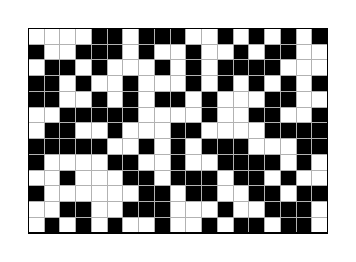
\begin{tikzpicture}[x=2mm,y=2mm]
\fill (4,12) rectangle +(1,1);\fill (5,12) rectangle +(1,1);\fill (7,12) rectangle +(1,1);\fill (8,12) rectangle +(1,1);\fill (9,12) rectangle +(1,1);\fill (12,12) rectangle +(1,1);\fill (14,12) rectangle +(1,1);\fill (16,12) rectangle +(1,1);\fill (18,12) rectangle +(1,1);
\fill (0,11) rectangle +(1,1);\fill (3,11) rectangle +(1,1);\fill (4,11) rectangle +(1,1);\fill (5,11) rectangle +(1,1);\fill (7,11) rectangle +(1,1);\fill (10,11) rectangle +(1,1);\fill (13,11) rectangle +(1,1);\fill (15,11) rectangle +(1,1);\fill (16,11) rectangle +(1,1);
\fill (1,10) rectangle +(1,1);\fill (2,10) rectangle +(1,1);\fill (4,10) rectangle +(1,1);\fill (8,10) rectangle +(1,1);\fill (10,10) rectangle +(1,1);\fill (12,10) rectangle +(1,1);\fill (13,10) rectangle +(1,1);\fill (14,10) rectangle +(1,1);\fill (15,10) rectangle +(1,1);
\fill (0,9) rectangle +(1,1);\fill (1,9) rectangle +(1,1);\fill (3,9) rectangle +(1,1);\fill (6,9) rectangle +(1,1);\fill (10,9) rectangle +(1,1);\fill (12,9) rectangle +(1,1);\fill (14,9) rectangle +(1,1);\fill (16,9) rectangle +(1,1);\fill (18,9) rectangle +(1,1);
\fill (0,8) rectangle +(1,1);\fill (1,8) rectangle +(1,1);\fill (4,8) rectangle +(1,1);\fill (6,8) rectangle +(1,1);\fill (8,8) rectangle +(1,1);\fill (9,8) rectangle +(1,1);\fill (11,8) rectangle +(1,1);\fill (15,8) rectangle +(1,1);\fill (16,8) rectangle +(1,1);
\fill (2,7) rectangle +(1,1);\fill (3,7) rectangle +(1,1);\fill (4,7) rectangle +(1,1);\fill (5,7) rectangle +(1,1);\fill (6,7) rectangle +(1,1);\fill (11,7) rectangle +(1,1);\fill (14,7) rectangle +(1,1);\fill (15,7) rectangle +(1,1);\fill (18,7) rectangle +(1,1);
\fill (1,6) rectangle +(1,1);\fill (2,6) rectangle +(1,1);\fill (5,6) rectangle +(1,1);\fill (9,6) rectangle +(1,1);\fill (10,6) rectangle +(1,1);\fill (15,6) rectangle +(1,1);\fill (16,6) rectangle +(1,1);\fill (17,6) rectangle +(1,1);\fill (18,6) rectangle +(1,1);
\fill (0,5) rectangle +(1,1);\fill (1,5) rectangle +(1,1);\fill (2,5) rectangle +(1,1);\fill (3,5) rectangle +(1,1);\fill (4,5) rectangle +(1,1);\fill (7,5) rectangle +(1,1);\fill (9,5) rectangle +(1,1);\fill (11,5) rectangle +(1,1);\fill (12,5) rectangle +(1,1);\fill (13,5) rectangle +(1,1);\fill (17,5) rectangle +(1,1);\fill (18,5) rectangle +(1,1);
\fill (0,4) rectangle +(1,1);\fill (5,4) rectangle +(1,1);\fill (6,4) rectangle +(1,1);\fill (9,4) rectangle +(1,1);\fill (12,4) rectangle +(1,1);\fill (13,4) rectangle +(1,1);\fill (14,4) rectangle +(1,1);\fill (15,4) rectangle +(1,1);\fill (17,4) rectangle +(1,1);
\fill (2,3) rectangle +(1,1);\fill (6,3) rectangle +(1,1);\fill (7,3) rectangle +(1,1);\fill (9,3) rectangle +(1,1);\fill (10,3) rectangle +(1,1);\fill (11,3) rectangle +(1,1);\fill (13,3) rectangle +(1,1);\fill (14,3) rectangle +(1,1);\fill (16,3) rectangle +(1,1);
\fill (0,2) rectangle +(1,1);\fill (7,2) rectangle +(1,1);\fill (8,2) rectangle +(1,1);\fill (10,2) rectangle +(1,1);\fill (11,2) rectangle +(1,1);\fill (14,2) rectangle +(1,1);\fill (15,2) rectangle +(1,1);\fill (17,2) rectangle +(1,1);\fill (18,2) rectangle +(1,1);
\fill (2,1) rectangle +(1,1);\fill (3,1) rectangle +(1,1);\fill (6,1) rectangle +(1,1);\fill (7,1) rectangle +(1,1);\fill (8,1) rectangle +(1,1);\fill (12,1) rectangle +(1,1);\fill (15,1) rectangle +(1,1);\fill (16,1) rectangle +(1,1);\fill (17,1) rectangle +(1,1);
\fill (1,0) rectangle +(1,1);\fill (3,0) rectangle +(1,1);\fill (5,0) rectangle +(1,1);\fill (8,0) rectangle +(1,1);\fill (11,0) rectangle +(1,1);\fill (13,0) rectangle +(1,1);\fill (14,0) rectangle +(1,1);\fill (16,0) rectangle +(1,1);\fill (17,0) rectangle +(1,1);
\draw[black!30,line width=0.3pt,step=1] (0,0) grid (19,13);
\draw[line width=0.4pt] (0,0) rectangle (19,13);
\end{tikzpicture}\\[3pt]
{\small (a) $z(13,19;3,3)\ge 120$}
\end{minipage}\hfill
\begin{minipage}[b]{0.32\textwidth}\centering
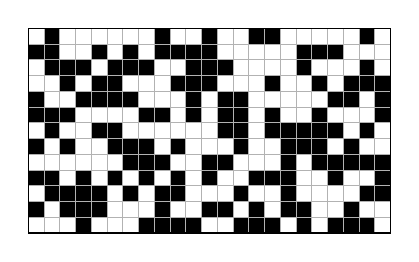
\begin{tikzpicture}[x=2mm,y=2mm]
\fill (1,12) rectangle +(1,1);\fill (8,12) rectangle +(1,1);\fill (11,12) rectangle +(1,1);\fill (14,12) rectangle +(1,1);\fill (15,12) rectangle +(1,1);\fill (21,12) rectangle +(1,1);
\fill (0,11) rectangle +(1,1);\fill (1,11) rectangle +(1,1);\fill (4,11) rectangle +(1,1);\fill (6,11) rectangle +(1,1);\fill (8,11) rectangle +(1,1);\fill (9,11) rectangle +(1,1);\fill (10,11) rectangle +(1,1);\fill (11,11) rectangle +(1,1);\fill (17,11) rectangle +(1,1);\fill (18,11) rectangle +(1,1);\fill (19,11) rectangle +(1,1);
\fill (1,10) rectangle +(1,1);\fill (2,10) rectangle +(1,1);\fill (3,10) rectangle +(1,1);\fill (5,10) rectangle +(1,1);\fill (6,10) rectangle +(1,1);\fill (7,10) rectangle +(1,1);\fill (10,10) rectangle +(1,1);\fill (11,10) rectangle +(1,1);\fill (12,10) rectangle +(1,1);\fill (17,10) rectangle +(1,1);\fill (21,10) rectangle +(1,1);
\fill (2,9) rectangle +(1,1);\fill (4,9) rectangle +(1,1);\fill (5,9) rectangle +(1,1);\fill (9,9) rectangle +(1,1);\fill (10,9) rectangle +(1,1);\fill (11,9) rectangle +(1,1);\fill (15,9) rectangle +(1,1);\fill (18,9) rectangle +(1,1);\fill (20,9) rectangle +(1,1);\fill (21,9) rectangle +(1,1);\fill (22,9) rectangle +(1,1);
\fill (0,8) rectangle +(1,1);\fill (3,8) rectangle +(1,1);\fill (4,8) rectangle +(1,1);\fill (5,8) rectangle +(1,1);\fill (6,8) rectangle +(1,1);\fill (10,8) rectangle +(1,1);\fill (12,8) rectangle +(1,1);\fill (13,8) rectangle +(1,1);\fill (19,8) rectangle +(1,1);\fill (20,8) rectangle +(1,1);\fill (22,8) rectangle +(1,1);
\fill (0,7) rectangle +(1,1);\fill (1,7) rectangle +(1,1);\fill (2,7) rectangle +(1,1);\fill (7,7) rectangle +(1,1);\fill (8,7) rectangle +(1,1);\fill (10,7) rectangle +(1,1);\fill (12,7) rectangle +(1,1);\fill (13,7) rectangle +(1,1);\fill (15,7) rectangle +(1,1);\fill (18,7) rectangle +(1,1);\fill (22,7) rectangle +(1,1);
\fill (1,6) rectangle +(1,1);\fill (4,6) rectangle +(1,1);\fill (5,6) rectangle +(1,1);\fill (12,6) rectangle +(1,1);\fill (13,6) rectangle +(1,1);\fill (15,6) rectangle +(1,1);\fill (16,6) rectangle +(1,1);\fill (17,6) rectangle +(1,1);\fill (18,6) rectangle +(1,1);\fill (19,6) rectangle +(1,1);\fill (21,6) rectangle +(1,1);
\fill (0,5) rectangle +(1,1);\fill (2,5) rectangle +(1,1);\fill (5,5) rectangle +(1,1);\fill (6,5) rectangle +(1,1);\fill (7,5) rectangle +(1,1);\fill (9,5) rectangle +(1,1);\fill (13,5) rectangle +(1,1);\fill (16,5) rectangle +(1,1);\fill (17,5) rectangle +(1,1);\fill (18,5) rectangle +(1,1);\fill (20,5) rectangle +(1,1);
\fill (6,4) rectangle +(1,1);\fill (7,4) rectangle +(1,1);\fill (8,4) rectangle +(1,1);\fill (11,4) rectangle +(1,1);\fill (12,4) rectangle +(1,1);\fill (16,4) rectangle +(1,1);\fill (18,4) rectangle +(1,1);\fill (19,4) rectangle +(1,1);\fill (20,4) rectangle +(1,1);\fill (21,4) rectangle +(1,1);\fill (22,4) rectangle +(1,1);
\fill (0,3) rectangle +(1,1);\fill (1,3) rectangle +(1,1);\fill (3,3) rectangle +(1,1);\fill (5,3) rectangle +(1,1);\fill (7,3) rectangle +(1,1);\fill (9,3) rectangle +(1,1);\fill (11,3) rectangle +(1,1);\fill (14,3) rectangle +(1,1);\fill (15,3) rectangle +(1,1);\fill (16,3) rectangle +(1,1);\fill (19,3) rectangle +(1,1);\fill (22,3) rectangle +(1,1);
\fill (1,2) rectangle +(1,1);\fill (2,2) rectangle +(1,1);\fill (3,2) rectangle +(1,1);\fill (4,2) rectangle +(1,1);\fill (6,2) rectangle +(1,1);\fill (8,2) rectangle +(1,1);\fill (9,2) rectangle +(1,1);\fill (13,2) rectangle +(1,1);\fill (16,2) rectangle +(1,1);\fill (21,2) rectangle +(1,1);\fill (22,2) rectangle +(1,1);
\fill (0,1) rectangle +(1,1);\fill (2,1) rectangle +(1,1);\fill (3,1) rectangle +(1,1);\fill (4,1) rectangle +(1,1);\fill (8,1) rectangle +(1,1);\fill (11,1) rectangle +(1,1);\fill (12,1) rectangle +(1,1);\fill (14,1) rectangle +(1,1);\fill (16,1) rectangle +(1,1);\fill (17,1) rectangle +(1,1);\fill (20,1) rectangle +(1,1);
\fill (3,0) rectangle +(1,1);\fill (7,0) rectangle +(1,1);\fill (8,0) rectangle +(1,1);\fill (9,0) rectangle +(1,1);\fill (10,0) rectangle +(1,1);\fill (13,0) rectangle +(1,1);\fill (14,0) rectangle +(1,1);\fill (15,0) rectangle +(1,1);\fill (17,0) rectangle +(1,1);\fill (19,0) rectangle +(1,1);\fill (20,0) rectangle +(1,1);\fill (21,0) rectangle +(1,1);
\draw[black!30,line width=0.3pt,step=1] (0,0) grid (23,13);
\draw[line width=0.4pt] (0,0) rectangle (23,13);
\end{tikzpicture}\\[3pt]
{\small (b) $z(13,23;3,3)\ge 140$}
\end{minipage}\hfill
\begin{minipage}[b]{0.32\textwidth}\centering
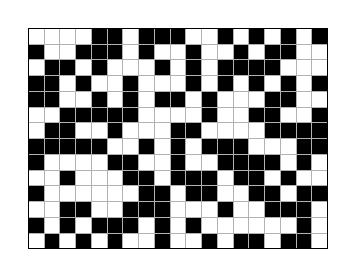
\begin{tikzpicture}[x=2mm,y=2mm]
\fill (4,13) rectangle +(1,1);\fill (5,13) rectangle +(1,1);\fill (7,13) rectangle +(1,1);\fill (8,13) rectangle +(1,1);\fill (9,13) rectangle +(1,1);\fill (12,13) rectangle +(1,1);\fill (14,13) rectangle +(1,1);\fill (16,13) rectangle +(1,1);\fill (18,13) rectangle +(1,1);
\fill (0,12) rectangle +(1,1);\fill (3,12) rectangle +(1,1);\fill (4,12) rectangle +(1,1);\fill (5,12) rectangle +(1,1);\fill (7,12) rectangle +(1,1);\fill (10,12) rectangle +(1,1);\fill (13,12) rectangle +(1,1);\fill (15,12) rectangle +(1,1);\fill (16,12) rectangle +(1,1);
\fill (1,11) rectangle +(1,1);\fill (2,11) rectangle +(1,1);\fill (4,11) rectangle +(1,1);\fill (8,11) rectangle +(1,1);\fill (10,11) rectangle +(1,1);\fill (12,11) rectangle +(1,1);\fill (13,11) rectangle +(1,1);\fill (14,11) rectangle +(1,1);\fill (15,11) rectangle +(1,1);
\fill (0,10) rectangle +(1,1);\fill (1,10) rectangle +(1,1);\fill (3,10) rectangle +(1,1);\fill (6,10) rectangle +(1,1);\fill (10,10) rectangle +(1,1);\fill (12,10) rectangle +(1,1);\fill (14,10) rectangle +(1,1);\fill (16,10) rectangle +(1,1);\fill (18,10) rectangle +(1,1);
\fill (0,9) rectangle +(1,1);\fill (1,9) rectangle +(1,1);\fill (4,9) rectangle +(1,1);\fill (6,9) rectangle +(1,1);\fill (8,9) rectangle +(1,1);\fill (9,9) rectangle +(1,1);\fill (11,9) rectangle +(1,1);\fill (15,9) rectangle +(1,1);\fill (16,9) rectangle +(1,1);
\fill (2,8) rectangle +(1,1);\fill (3,8) rectangle +(1,1);\fill (4,8) rectangle +(1,1);\fill (5,8) rectangle +(1,1);\fill (6,8) rectangle +(1,1);\fill (11,8) rectangle +(1,1);\fill (14,8) rectangle +(1,1);\fill (15,8) rectangle +(1,1);\fill (18,8) rectangle +(1,1);
\fill (1,7) rectangle +(1,1);\fill (2,7) rectangle +(1,1);\fill (5,7) rectangle +(1,1);\fill (9,7) rectangle +(1,1);\fill (10,7) rectangle +(1,1);\fill (15,7) rectangle +(1,1);\fill (16,7) rectangle +(1,1);\fill (17,7) rectangle +(1,1);\fill (18,7) rectangle +(1,1);
\fill (0,6) rectangle +(1,1);\fill (1,6) rectangle +(1,1);\fill (2,6) rectangle +(1,1);\fill (3,6) rectangle +(1,1);\fill (4,6) rectangle +(1,1);\fill (7,6) rectangle +(1,1);\fill (9,6) rectangle +(1,1);\fill (11,6) rectangle +(1,1);\fill (12,6) rectangle +(1,1);\fill (13,6) rectangle +(1,1);\fill (17,6) rectangle +(1,1);\fill (18,6) rectangle +(1,1);
\fill (0,5) rectangle +(1,1);\fill (5,5) rectangle +(1,1);\fill (6,5) rectangle +(1,1);\fill (9,5) rectangle +(1,1);\fill (12,5) rectangle +(1,1);\fill (13,5) rectangle +(1,1);\fill (14,5) rectangle +(1,1);\fill (15,5) rectangle +(1,1);\fill (17,5) rectangle +(1,1);
\fill (2,4) rectangle +(1,1);\fill (6,4) rectangle +(1,1);\fill (7,4) rectangle +(1,1);\fill (9,4) rectangle +(1,1);\fill (10,4) rectangle +(1,1);\fill (11,4) rectangle +(1,1);\fill (13,4) rectangle +(1,1);\fill (14,4) rectangle +(1,1);\fill (16,4) rectangle +(1,1);
\fill (0,3) rectangle +(1,1);\fill (7,3) rectangle +(1,1);\fill (8,3) rectangle +(1,1);\fill (10,3) rectangle +(1,1);\fill (11,3) rectangle +(1,1);\fill (14,3) rectangle +(1,1);\fill (15,3) rectangle +(1,1);\fill (17,3) rectangle +(1,1);\fill (18,3) rectangle +(1,1);
\fill (2,2) rectangle +(1,1);\fill (3,2) rectangle +(1,1);\fill (6,2) rectangle +(1,1);\fill (7,2) rectangle +(1,1);\fill (8,2) rectangle +(1,1);\fill (12,2) rectangle +(1,1);\fill (15,2) rectangle +(1,1);\fill (16,2) rectangle +(1,1);\fill (17,2) rectangle +(1,1);
\fill (0,1) rectangle +(1,1);\fill (2,1) rectangle +(1,1);\fill (4,1) rectangle +(1,1);\fill (5,1) rectangle +(1,1);\fill (6,1) rectangle +(1,1);\fill (8,1) rectangle +(1,1);\fill (10,1) rectangle +(1,1);\fill (17,1) rectangle +(1,1);
\fill (1,0) rectangle +(1,1);\fill (3,0) rectangle +(1,1);\fill (5,0) rectangle +(1,1);\fill (8,0) rectangle +(1,1);\fill (11,0) rectangle +(1,1);\fill (13,0) rectangle +(1,1);\fill (14,0) rectangle +(1,1);\fill (16,0) rectangle +(1,1);\fill (17,0) rectangle +(1,1);
\draw[black!30,line width=0.3pt,step=1] (0,0) grid (19,14);
\draw[line width=0.4pt] (0,0) rectangle (19,14);
\end{tikzpicture}\\[3pt]
{\small (c) $z(14,19;3,3)\ge 128$}
\end{minipage}

\bigskip
\begin{minipage}[b]{0.32\textwidth}\centering
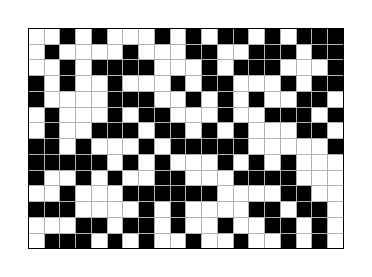
\begin{tikzpicture}[x=2mm,y=2mm]
\fill (2,13) rectangle +(1,1);\fill (4,13) rectangle +(1,1);\fill (8,13) rectangle +(1,1);\fill (10,13) rectangle +(1,1);\fill (12,13) rectangle +(1,1);\fill (13,13) rectangle +(1,1);\fill (15,13) rectangle +(1,1);\fill (17,13) rectangle +(1,1);\fill (18,13) rectangle +(1,1);\fill (19,13) rectangle +(1,1);
\fill (1,12) rectangle +(1,1);\fill (6,12) rectangle +(1,1);\fill (10,12) rectangle +(1,1);\fill (11,12) rectangle +(1,1);\fill (14,12) rectangle +(1,1);\fill (15,12) rectangle +(1,1);\fill (16,12) rectangle +(1,1);\fill (18,12) rectangle +(1,1);\fill (19,12) rectangle +(1,1);
\fill (2,11) rectangle +(1,1);\fill (4,11) rectangle +(1,1);\fill (5,11) rectangle +(1,1);\fill (6,11) rectangle +(1,1);\fill (7,11) rectangle +(1,1);\fill (11,11) rectangle +(1,1);\fill (13,11) rectangle +(1,1);\fill (14,11) rectangle +(1,1);\fill (15,11) rectangle +(1,1);\fill (19,11) rectangle +(1,1);
\fill (0,10) rectangle +(1,1);\fill (2,10) rectangle +(1,1);\fill (5,10) rectangle +(1,1);\fill (9,10) rectangle +(1,1);\fill (11,10) rectangle +(1,1);\fill (12,10) rectangle +(1,1);\fill (16,10) rectangle +(1,1);\fill (18,10) rectangle +(1,1);\fill (19,10) rectangle +(1,1);
\fill (0,9) rectangle +(1,1);\fill (5,9) rectangle +(1,1);\fill (6,9) rectangle +(1,1);\fill (7,9) rectangle +(1,1);\fill (10,9) rectangle +(1,1);\fill (12,9) rectangle +(1,1);\fill (14,9) rectangle +(1,1);\fill (17,9) rectangle +(1,1);\fill (18,9) rectangle +(1,1);
\fill (1,8) rectangle +(1,1);\fill (5,8) rectangle +(1,1);\fill (7,8) rectangle +(1,1);\fill (8,8) rectangle +(1,1);\fill (12,8) rectangle +(1,1);\fill (15,8) rectangle +(1,1);\fill (16,8) rectangle +(1,1);\fill (17,8) rectangle +(1,1);\fill (19,8) rectangle +(1,1);
\fill (1,7) rectangle +(1,1);\fill (4,7) rectangle +(1,1);\fill (5,7) rectangle +(1,1);\fill (6,7) rectangle +(1,1);\fill (8,7) rectangle +(1,1);\fill (9,7) rectangle +(1,1);\fill (11,7) rectangle +(1,1);\fill (13,7) rectangle +(1,1);\fill (17,7) rectangle +(1,1);\fill (18,7) rectangle +(1,1);
\fill (0,6) rectangle +(1,1);\fill (1,6) rectangle +(1,1);\fill (3,6) rectangle +(1,1);\fill (7,6) rectangle +(1,1);\fill (9,6) rectangle +(1,1);\fill (10,6) rectangle +(1,1);\fill (11,6) rectangle +(1,1);\fill (12,6) rectangle +(1,1);\fill (13,6) rectangle +(1,1);\fill (19,6) rectangle +(1,1);
\fill (0,5) rectangle +(1,1);\fill (1,5) rectangle +(1,1);\fill (2,5) rectangle +(1,1);\fill (3,5) rectangle +(1,1);\fill (4,5) rectangle +(1,1);\fill (6,5) rectangle +(1,1);\fill (8,5) rectangle +(1,1);\fill (12,5) rectangle +(1,1);\fill (14,5) rectangle +(1,1);\fill (16,5) rectangle +(1,1);
\fill (0,4) rectangle +(1,1);\fill (3,4) rectangle +(1,1);\fill (5,4) rectangle +(1,1);\fill (8,4) rectangle +(1,1);\fill (9,4) rectangle +(1,1);\fill (13,4) rectangle +(1,1);\fill (14,4) rectangle +(1,1);\fill (15,4) rectangle +(1,1);\fill (16,4) rectangle +(1,1);
\fill (2,3) rectangle +(1,1);\fill (6,3) rectangle +(1,1);\fill (7,3) rectangle +(1,1);\fill (8,3) rectangle +(1,1);\fill (9,3) rectangle +(1,1);\fill (10,3) rectangle +(1,1);\fill (11,3) rectangle +(1,1);\fill (16,3) rectangle +(1,1);\fill (17,3) rectangle +(1,1);
\fill (0,2) rectangle +(1,1);\fill (1,2) rectangle +(1,1);\fill (2,2) rectangle +(1,1);\fill (7,2) rectangle +(1,1);\fill (9,2) rectangle +(1,1);\fill (14,2) rectangle +(1,1);\fill (15,2) rectangle +(1,1);\fill (17,2) rectangle +(1,1);\fill (18,2) rectangle +(1,1);
\fill (3,1) rectangle +(1,1);\fill (4,1) rectangle +(1,1);\fill (6,1) rectangle +(1,1);\fill (7,1) rectangle +(1,1);\fill (9,1) rectangle +(1,1);\fill (12,1) rectangle +(1,1);\fill (15,1) rectangle +(1,1);\fill (16,1) rectangle +(1,1);\fill (18,1) rectangle +(1,1);
\fill (1,0) rectangle +(1,1);\fill (2,0) rectangle +(1,1);\fill (3,0) rectangle +(1,1);\fill (5,0) rectangle +(1,1);\fill (7,0) rectangle +(1,1);\fill (10,0) rectangle +(1,1);\fill (13,0) rectangle +(1,1);\fill (16,0) rectangle +(1,1);\fill (18,0) rectangle +(1,1);
\draw[black!30,line width=0.3pt,step=1] (0,0) grid (20,14);
\draw[line width=0.4pt] (0,0) rectangle (20,14);
\end{tikzpicture}\\[3pt]
{\small (d) $z(14,20;3,3)\ge 131$}
\end{minipage}\hfill
\begin{minipage}[b]{0.32\textwidth}\centering
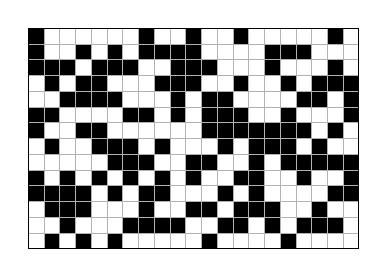
\begin{tikzpicture}[x=2mm,y=2mm]
\fill (0,13) rectangle +(1,1);\fill (7,13) rectangle +(1,1);\fill (10,13) rectangle +(1,1);\fill (13,13) rectangle +(1,1);\fill (19,13) rectangle +(1,1);
\fill (0,12) rectangle +(1,1);\fill (3,12) rectangle +(1,1);\fill (5,12) rectangle +(1,1);\fill (7,12) rectangle +(1,1);\fill (8,12) rectangle +(1,1);\fill (9,12) rectangle +(1,1);\fill (10,12) rectangle +(1,1);\fill (15,12) rectangle +(1,1);\fill (16,12) rectangle +(1,1);\fill (17,12) rectangle +(1,1);
\fill (0,11) rectangle +(1,1);\fill (1,11) rectangle +(1,1);\fill (2,11) rectangle +(1,1);\fill (4,11) rectangle +(1,1);\fill (5,11) rectangle +(1,1);\fill (6,11) rectangle +(1,1);\fill (9,11) rectangle +(1,1);\fill (10,11) rectangle +(1,1);\fill (11,11) rectangle +(1,1);\fill (15,11) rectangle +(1,1);\fill (19,11) rectangle +(1,1);
\fill (1,10) rectangle +(1,1);\fill (3,10) rectangle +(1,1);\fill (4,10) rectangle +(1,1);\fill (8,10) rectangle +(1,1);\fill (9,10) rectangle +(1,1);\fill (10,10) rectangle +(1,1);\fill (13,10) rectangle +(1,1);\fill (16,10) rectangle +(1,1);\fill (18,10) rectangle +(1,1);\fill (19,10) rectangle +(1,1);\fill (20,10) rectangle +(1,1);
\fill (2,9) rectangle +(1,1);\fill (3,9) rectangle +(1,1);\fill (4,9) rectangle +(1,1);\fill (5,9) rectangle +(1,1);\fill (9,9) rectangle +(1,1);\fill (11,9) rectangle +(1,1);\fill (12,9) rectangle +(1,1);\fill (17,9) rectangle +(1,1);\fill (18,9) rectangle +(1,1);\fill (20,9) rectangle +(1,1);
\fill (0,8) rectangle +(1,1);\fill (1,8) rectangle +(1,1);\fill (6,8) rectangle +(1,1);\fill (7,8) rectangle +(1,1);\fill (9,8) rectangle +(1,1);\fill (11,8) rectangle +(1,1);\fill (12,8) rectangle +(1,1);\fill (13,8) rectangle +(1,1);\fill (16,8) rectangle +(1,1);\fill (20,8) rectangle +(1,1);
\fill (0,7) rectangle +(1,1);\fill (3,7) rectangle +(1,1);\fill (4,7) rectangle +(1,1);\fill (11,7) rectangle +(1,1);\fill (12,7) rectangle +(1,1);\fill (13,7) rectangle +(1,1);\fill (14,7) rectangle +(1,1);\fill (15,7) rectangle +(1,1);\fill (16,7) rectangle +(1,1);\fill (17,7) rectangle +(1,1);\fill (19,7) rectangle +(1,1);
\fill (1,6) rectangle +(1,1);\fill (4,6) rectangle +(1,1);\fill (5,6) rectangle +(1,1);\fill (6,6) rectangle +(1,1);\fill (8,6) rectangle +(1,1);\fill (12,6) rectangle +(1,1);\fill (14,6) rectangle +(1,1);\fill (15,6) rectangle +(1,1);\fill (16,6) rectangle +(1,1);\fill (18,6) rectangle +(1,1);
\fill (5,5) rectangle +(1,1);\fill (6,5) rectangle +(1,1);\fill (7,5) rectangle +(1,1);\fill (10,5) rectangle +(1,1);\fill (11,5) rectangle +(1,1);\fill (14,5) rectangle +(1,1);\fill (16,5) rectangle +(1,1);\fill (17,5) rectangle +(1,1);\fill (18,5) rectangle +(1,1);\fill (19,5) rectangle +(1,1);\fill (20,5) rectangle +(1,1);
\fill (0,4) rectangle +(1,1);\fill (2,4) rectangle +(1,1);\fill (4,4) rectangle +(1,1);\fill (6,4) rectangle +(1,1);\fill (8,4) rectangle +(1,1);\fill (10,4) rectangle +(1,1);\fill (13,4) rectangle +(1,1);\fill (14,4) rectangle +(1,1);\fill (17,4) rectangle +(1,1);\fill (20,4) rectangle +(1,1);
\fill (0,3) rectangle +(1,1);\fill (1,3) rectangle +(1,1);\fill (2,3) rectangle +(1,1);\fill (3,3) rectangle +(1,1);\fill (5,3) rectangle +(1,1);\fill (7,3) rectangle +(1,1);\fill (8,3) rectangle +(1,1);\fill (12,3) rectangle +(1,1);\fill (14,3) rectangle +(1,1);\fill (19,3) rectangle +(1,1);\fill (20,3) rectangle +(1,1);
\fill (1,2) rectangle +(1,1);\fill (2,2) rectangle +(1,1);\fill (3,2) rectangle +(1,1);\fill (7,2) rectangle +(1,1);\fill (10,2) rectangle +(1,1);\fill (11,2) rectangle +(1,1);\fill (13,2) rectangle +(1,1);\fill (14,2) rectangle +(1,1);\fill (15,2) rectangle +(1,1);\fill (18,2) rectangle +(1,1);
\fill (2,1) rectangle +(1,1);\fill (6,1) rectangle +(1,1);\fill (7,1) rectangle +(1,1);\fill (8,1) rectangle +(1,1);\fill (9,1) rectangle +(1,1);\fill (12,1) rectangle +(1,1);\fill (13,1) rectangle +(1,1);\fill (15,1) rectangle +(1,1);\fill (17,1) rectangle +(1,1);\fill (18,1) rectangle +(1,1);\fill (19,1) rectangle +(1,1);
\fill (1,0) rectangle +(1,1);\fill (3,0) rectangle +(1,1);\fill (5,0) rectangle +(1,1);\fill (11,0) rectangle +(1,1);\fill (16,0) rectangle +(1,1);
\draw[black!30,line width=0.3pt,step=1] (0,0) grid (21,14);
\draw[line width=0.4pt] (0,0) rectangle (21,14);
\end{tikzpicture}\\[3pt]
{\small (e) $z(14,21;3,3)\ge 136$}
\end{minipage}\hfill
\begin{minipage}[b]{0.32\textwidth}\centering
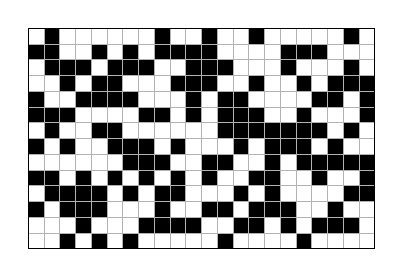
\begin{tikzpicture}[x=2mm,y=2mm]
\fill (1,13) rectangle +(1,1);\fill (8,13) rectangle +(1,1);\fill (11,13) rectangle +(1,1);\fill (14,13) rectangle +(1,1);\fill (20,13) rectangle +(1,1);
\fill (0,12) rectangle +(1,1);\fill (1,12) rectangle +(1,1);\fill (4,12) rectangle +(1,1);\fill (6,12) rectangle +(1,1);\fill (8,12) rectangle +(1,1);\fill (9,12) rectangle +(1,1);\fill (10,12) rectangle +(1,1);\fill (11,12) rectangle +(1,1);\fill (16,12) rectangle +(1,1);\fill (17,12) rectangle +(1,1);\fill (18,12) rectangle +(1,1);
\fill (1,11) rectangle +(1,1);\fill (2,11) rectangle +(1,1);\fill (3,11) rectangle +(1,1);\fill (5,11) rectangle +(1,1);\fill (6,11) rectangle +(1,1);\fill (7,11) rectangle +(1,1);\fill (10,11) rectangle +(1,1);\fill (11,11) rectangle +(1,1);\fill (12,11) rectangle +(1,1);\fill (16,11) rectangle +(1,1);\fill (20,11) rectangle +(1,1);
\fill (2,10) rectangle +(1,1);\fill (4,10) rectangle +(1,1);\fill (5,10) rectangle +(1,1);\fill (9,10) rectangle +(1,1);\fill (10,10) rectangle +(1,1);\fill (11,10) rectangle +(1,1);\fill (14,10) rectangle +(1,1);\fill (17,10) rectangle +(1,1);\fill (19,10) rectangle +(1,1);\fill (20,10) rectangle +(1,1);\fill (21,10) rectangle +(1,1);
\fill (0,9) rectangle +(1,1);\fill (3,9) rectangle +(1,1);\fill (4,9) rectangle +(1,1);\fill (5,9) rectangle +(1,1);\fill (6,9) rectangle +(1,1);\fill (10,9) rectangle +(1,1);\fill (12,9) rectangle +(1,1);\fill (13,9) rectangle +(1,1);\fill (18,9) rectangle +(1,1);\fill (19,9) rectangle +(1,1);\fill (21,9) rectangle +(1,1);
\fill (0,8) rectangle +(1,1);\fill (1,8) rectangle +(1,1);\fill (2,8) rectangle +(1,1);\fill (7,8) rectangle +(1,1);\fill (8,8) rectangle +(1,1);\fill (10,8) rectangle +(1,1);\fill (12,8) rectangle +(1,1);\fill (13,8) rectangle +(1,1);\fill (14,8) rectangle +(1,1);\fill (17,8) rectangle +(1,1);\fill (21,8) rectangle +(1,1);
\fill (1,7) rectangle +(1,1);\fill (4,7) rectangle +(1,1);\fill (5,7) rectangle +(1,1);\fill (12,7) rectangle +(1,1);\fill (13,7) rectangle +(1,1);\fill (14,7) rectangle +(1,1);\fill (15,7) rectangle +(1,1);\fill (16,7) rectangle +(1,1);\fill (17,7) rectangle +(1,1);\fill (18,7) rectangle +(1,1);\fill (20,7) rectangle +(1,1);
\fill (0,6) rectangle +(1,1);\fill (2,6) rectangle +(1,1);\fill (5,6) rectangle +(1,1);\fill (6,6) rectangle +(1,1);\fill (7,6) rectangle +(1,1);\fill (9,6) rectangle +(1,1);\fill (13,6) rectangle +(1,1);\fill (15,6) rectangle +(1,1);\fill (16,6) rectangle +(1,1);\fill (17,6) rectangle +(1,1);\fill (19,6) rectangle +(1,1);
\fill (6,5) rectangle +(1,1);\fill (7,5) rectangle +(1,1);\fill (8,5) rectangle +(1,1);\fill (11,5) rectangle +(1,1);\fill (12,5) rectangle +(1,1);\fill (15,5) rectangle +(1,1);\fill (17,5) rectangle +(1,1);\fill (18,5) rectangle +(1,1);\fill (19,5) rectangle +(1,1);\fill (20,5) rectangle +(1,1);\fill (21,5) rectangle +(1,1);
\fill (0,4) rectangle +(1,1);\fill (1,4) rectangle +(1,1);\fill (3,4) rectangle +(1,1);\fill (5,4) rectangle +(1,1);\fill (7,4) rectangle +(1,1);\fill (9,4) rectangle +(1,1);\fill (11,4) rectangle +(1,1);\fill (14,4) rectangle +(1,1);\fill (15,4) rectangle +(1,1);\fill (18,4) rectangle +(1,1);\fill (21,4) rectangle +(1,1);
\fill (1,3) rectangle +(1,1);\fill (2,3) rectangle +(1,1);\fill (3,3) rectangle +(1,1);\fill (4,3) rectangle +(1,1);\fill (6,3) rectangle +(1,1);\fill (8,3) rectangle +(1,1);\fill (9,3) rectangle +(1,1);\fill (13,3) rectangle +(1,1);\fill (15,3) rectangle +(1,1);\fill (20,3) rectangle +(1,1);\fill (21,3) rectangle +(1,1);
\fill (0,2) rectangle +(1,1);\fill (2,2) rectangle +(1,1);\fill (3,2) rectangle +(1,1);\fill (4,2) rectangle +(1,1);\fill (8,2) rectangle +(1,1);\fill (11,2) rectangle +(1,1);\fill (12,2) rectangle +(1,1);\fill (14,2) rectangle +(1,1);\fill (15,2) rectangle +(1,1);\fill (16,2) rectangle +(1,1);\fill (19,2) rectangle +(1,1);
\fill (3,1) rectangle +(1,1);\fill (7,1) rectangle +(1,1);\fill (8,1) rectangle +(1,1);\fill (9,1) rectangle +(1,1);\fill (10,1) rectangle +(1,1);\fill (13,1) rectangle +(1,1);\fill (14,1) rectangle +(1,1);\fill (16,1) rectangle +(1,1);\fill (18,1) rectangle +(1,1);\fill (19,1) rectangle +(1,1);\fill (20,1) rectangle +(1,1);
\fill (2,0) rectangle +(1,1);\fill (4,0) rectangle +(1,1);\fill (6,0) rectangle +(1,1);\fill (12,0) rectangle +(1,1);\fill (17,0) rectangle +(1,1);
\draw[black!30,line width=0.3pt,step=1] (0,0) grid (22,14);
\draw[line width=0.4pt] (0,0) rectangle (22,14);
\end{tikzpicture}\\[3pt]
{\small (f) $z(14,22;3,3)\ge 142$}
\end{minipage}

\bigskip
\begin{minipage}[b]{0.32\textwidth}\centering
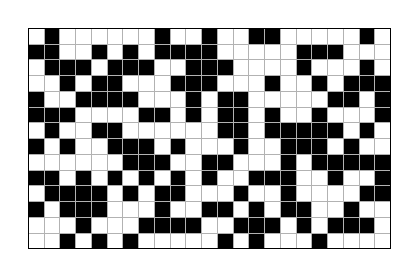
\begin{tikzpicture}[x=2mm,y=2mm]
\fill (1,13) rectangle +(1,1);\fill (8,13) rectangle +(1,1);\fill (11,13) rectangle +(1,1);\fill (14,13) rectangle +(1,1);\fill (15,13) rectangle +(1,1);\fill (21,13) rectangle +(1,1);
\fill (0,12) rectangle +(1,1);\fill (1,12) rectangle +(1,1);\fill (4,12) rectangle +(1,1);\fill (6,12) rectangle +(1,1);\fill (8,12) rectangle +(1,1);\fill (9,12) rectangle +(1,1);\fill (10,12) rectangle +(1,1);\fill (11,12) rectangle +(1,1);\fill (17,12) rectangle +(1,1);\fill (18,12) rectangle +(1,1);\fill (19,12) rectangle +(1,1);
\fill (1,11) rectangle +(1,1);\fill (2,11) rectangle +(1,1);\fill (3,11) rectangle +(1,1);\fill (5,11) rectangle +(1,1);\fill (6,11) rectangle +(1,1);\fill (7,11) rectangle +(1,1);\fill (10,11) rectangle +(1,1);\fill (11,11) rectangle +(1,1);\fill (12,11) rectangle +(1,1);\fill (17,11) rectangle +(1,1);\fill (21,11) rectangle +(1,1);
\fill (2,10) rectangle +(1,1);\fill (4,10) rectangle +(1,1);\fill (5,10) rectangle +(1,1);\fill (9,10) rectangle +(1,1);\fill (10,10) rectangle +(1,1);\fill (11,10) rectangle +(1,1);\fill (15,10) rectangle +(1,1);\fill (18,10) rectangle +(1,1);\fill (20,10) rectangle +(1,1);\fill (21,10) rectangle +(1,1);\fill (22,10) rectangle +(1,1);
\fill (0,9) rectangle +(1,1);\fill (3,9) rectangle +(1,1);\fill (4,9) rectangle +(1,1);\fill (5,9) rectangle +(1,1);\fill (6,9) rectangle +(1,1);\fill (10,9) rectangle +(1,1);\fill (12,9) rectangle +(1,1);\fill (13,9) rectangle +(1,1);\fill (19,9) rectangle +(1,1);\fill (20,9) rectangle +(1,1);\fill (22,9) rectangle +(1,1);
\fill (0,8) rectangle +(1,1);\fill (1,8) rectangle +(1,1);\fill (2,8) rectangle +(1,1);\fill (7,8) rectangle +(1,1);\fill (8,8) rectangle +(1,1);\fill (10,8) rectangle +(1,1);\fill (12,8) rectangle +(1,1);\fill (13,8) rectangle +(1,1);\fill (15,8) rectangle +(1,1);\fill (18,8) rectangle +(1,1);\fill (22,8) rectangle +(1,1);
\fill (1,7) rectangle +(1,1);\fill (4,7) rectangle +(1,1);\fill (5,7) rectangle +(1,1);\fill (12,7) rectangle +(1,1);\fill (13,7) rectangle +(1,1);\fill (15,7) rectangle +(1,1);\fill (16,7) rectangle +(1,1);\fill (17,7) rectangle +(1,1);\fill (18,7) rectangle +(1,1);\fill (19,7) rectangle +(1,1);\fill (21,7) rectangle +(1,1);
\fill (0,6) rectangle +(1,1);\fill (2,6) rectangle +(1,1);\fill (5,6) rectangle +(1,1);\fill (6,6) rectangle +(1,1);\fill (7,6) rectangle +(1,1);\fill (9,6) rectangle +(1,1);\fill (13,6) rectangle +(1,1);\fill (16,6) rectangle +(1,1);\fill (17,6) rectangle +(1,1);\fill (18,6) rectangle +(1,1);\fill (20,6) rectangle +(1,1);
\fill (6,5) rectangle +(1,1);\fill (7,5) rectangle +(1,1);\fill (8,5) rectangle +(1,1);\fill (11,5) rectangle +(1,1);\fill (12,5) rectangle +(1,1);\fill (16,5) rectangle +(1,1);\fill (18,5) rectangle +(1,1);\fill (19,5) rectangle +(1,1);\fill (20,5) rectangle +(1,1);\fill (21,5) rectangle +(1,1);\fill (22,5) rectangle +(1,1);
\fill (0,4) rectangle +(1,1);\fill (1,4) rectangle +(1,1);\fill (3,4) rectangle +(1,1);\fill (5,4) rectangle +(1,1);\fill (7,4) rectangle +(1,1);\fill (9,4) rectangle +(1,1);\fill (11,4) rectangle +(1,1);\fill (14,4) rectangle +(1,1);\fill (15,4) rectangle +(1,1);\fill (16,4) rectangle +(1,1);\fill (19,4) rectangle +(1,1);\fill (22,4) rectangle +(1,1);
\fill (1,3) rectangle +(1,1);\fill (2,3) rectangle +(1,1);\fill (3,3) rectangle +(1,1);\fill (4,3) rectangle +(1,1);\fill (6,3) rectangle +(1,1);\fill (8,3) rectangle +(1,1);\fill (9,3) rectangle +(1,1);\fill (13,3) rectangle +(1,1);\fill (16,3) rectangle +(1,1);\fill (21,3) rectangle +(1,1);\fill (22,3) rectangle +(1,1);
\fill (0,2) rectangle +(1,1);\fill (2,2) rectangle +(1,1);\fill (3,2) rectangle +(1,1);\fill (4,2) rectangle +(1,1);\fill (8,2) rectangle +(1,1);\fill (11,2) rectangle +(1,1);\fill (12,2) rectangle +(1,1);\fill (14,2) rectangle +(1,1);\fill (16,2) rectangle +(1,1);\fill (17,2) rectangle +(1,1);\fill (20,2) rectangle +(1,1);
\fill (3,1) rectangle +(1,1);\fill (7,1) rectangle +(1,1);\fill (8,1) rectangle +(1,1);\fill (9,1) rectangle +(1,1);\fill (10,1) rectangle +(1,1);\fill (13,1) rectangle +(1,1);\fill (14,1) rectangle +(1,1);\fill (15,1) rectangle +(1,1);\fill (17,1) rectangle +(1,1);\fill (19,1) rectangle +(1,1);\fill (20,1) rectangle +(1,1);\fill (21,1) rectangle +(1,1);
\fill (2,0) rectangle +(1,1);\fill (4,0) rectangle +(1,1);\fill (6,0) rectangle +(1,1);\fill (12,0) rectangle +(1,1);\fill (14,0) rectangle +(1,1);\fill (18,0) rectangle +(1,1);
\draw[black!30,line width=0.3pt,step=1] (0,0) grid (23,14);
\draw[line width=0.4pt] (0,0) rectangle (23,14);
\end{tikzpicture}\\[3pt]
{\small (g) $z(14,23;3,3)\ge 146$}
\end{minipage}\hfill
\begin{minipage}[b]{0.32\textwidth}\centering
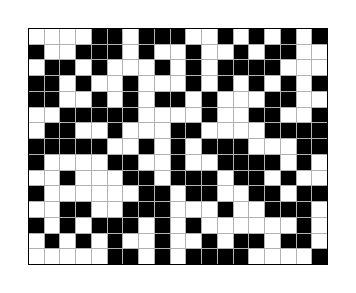
\begin{tikzpicture}[x=2mm,y=2mm]
\fill (4,14) rectangle +(1,1);\fill (5,14) rectangle +(1,1);\fill (7,14) rectangle +(1,1);\fill (8,14) rectangle +(1,1);\fill (9,14) rectangle +(1,1);\fill (12,14) rectangle +(1,1);\fill (14,14) rectangle +(1,1);\fill (16,14) rectangle +(1,1);\fill (18,14) rectangle +(1,1);
\fill (0,13) rectangle +(1,1);\fill (3,13) rectangle +(1,1);\fill (4,13) rectangle +(1,1);\fill (5,13) rectangle +(1,1);\fill (7,13) rectangle +(1,1);\fill (10,13) rectangle +(1,1);\fill (13,13) rectangle +(1,1);\fill (15,13) rectangle +(1,1);\fill (16,13) rectangle +(1,1);
\fill (1,12) rectangle +(1,1);\fill (2,12) rectangle +(1,1);\fill (4,12) rectangle +(1,1);\fill (8,12) rectangle +(1,1);\fill (10,12) rectangle +(1,1);\fill (12,12) rectangle +(1,1);\fill (13,12) rectangle +(1,1);\fill (14,12) rectangle +(1,1);\fill (15,12) rectangle +(1,1);
\fill (0,11) rectangle +(1,1);\fill (1,11) rectangle +(1,1);\fill (3,11) rectangle +(1,1);\fill (6,11) rectangle +(1,1);\fill (10,11) rectangle +(1,1);\fill (12,11) rectangle +(1,1);\fill (14,11) rectangle +(1,1);\fill (16,11) rectangle +(1,1);\fill (18,11) rectangle +(1,1);
\fill (0,10) rectangle +(1,1);\fill (1,10) rectangle +(1,1);\fill (4,10) rectangle +(1,1);\fill (6,10) rectangle +(1,1);\fill (8,10) rectangle +(1,1);\fill (9,10) rectangle +(1,1);\fill (11,10) rectangle +(1,1);\fill (15,10) rectangle +(1,1);\fill (16,10) rectangle +(1,1);
\fill (2,9) rectangle +(1,1);\fill (3,9) rectangle +(1,1);\fill (4,9) rectangle +(1,1);\fill (5,9) rectangle +(1,1);\fill (6,9) rectangle +(1,1);\fill (11,9) rectangle +(1,1);\fill (14,9) rectangle +(1,1);\fill (15,9) rectangle +(1,1);\fill (18,9) rectangle +(1,1);
\fill (1,8) rectangle +(1,1);\fill (2,8) rectangle +(1,1);\fill (5,8) rectangle +(1,1);\fill (9,8) rectangle +(1,1);\fill (10,8) rectangle +(1,1);\fill (15,8) rectangle +(1,1);\fill (16,8) rectangle +(1,1);\fill (17,8) rectangle +(1,1);\fill (18,8) rectangle +(1,1);
\fill (0,7) rectangle +(1,1);\fill (1,7) rectangle +(1,1);\fill (2,7) rectangle +(1,1);\fill (3,7) rectangle +(1,1);\fill (4,7) rectangle +(1,1);\fill (7,7) rectangle +(1,1);\fill (9,7) rectangle +(1,1);\fill (11,7) rectangle +(1,1);\fill (12,7) rectangle +(1,1);\fill (13,7) rectangle +(1,1);\fill (17,7) rectangle +(1,1);\fill (18,7) rectangle +(1,1);
\fill (0,6) rectangle +(1,1);\fill (5,6) rectangle +(1,1);\fill (6,6) rectangle +(1,1);\fill (9,6) rectangle +(1,1);\fill (12,6) rectangle +(1,1);\fill (13,6) rectangle +(1,1);\fill (14,6) rectangle +(1,1);\fill (15,6) rectangle +(1,1);\fill (17,6) rectangle +(1,1);
\fill (2,5) rectangle +(1,1);\fill (6,5) rectangle +(1,1);\fill (7,5) rectangle +(1,1);\fill (9,5) rectangle +(1,1);\fill (10,5) rectangle +(1,1);\fill (11,5) rectangle +(1,1);\fill (13,5) rectangle +(1,1);\fill (14,5) rectangle +(1,1);\fill (16,5) rectangle +(1,1);
\fill (0,4) rectangle +(1,1);\fill (7,4) rectangle +(1,1);\fill (8,4) rectangle +(1,1);\fill (10,4) rectangle +(1,1);\fill (11,4) rectangle +(1,1);\fill (14,4) rectangle +(1,1);\fill (15,4) rectangle +(1,1);\fill (17,4) rectangle +(1,1);\fill (18,4) rectangle +(1,1);
\fill (2,3) rectangle +(1,1);\fill (3,3) rectangle +(1,1);\fill (6,3) rectangle +(1,1);\fill (7,3) rectangle +(1,1);\fill (8,3) rectangle +(1,1);\fill (12,3) rectangle +(1,1);\fill (15,3) rectangle +(1,1);\fill (16,3) rectangle +(1,1);\fill (17,3) rectangle +(1,1);
\fill (0,2) rectangle +(1,1);\fill (2,2) rectangle +(1,1);\fill (4,2) rectangle +(1,1);\fill (5,2) rectangle +(1,1);\fill (6,2) rectangle +(1,1);\fill (8,2) rectangle +(1,1);\fill (10,2) rectangle +(1,1);\fill (17,2) rectangle +(1,1);
\fill (1,1) rectangle +(1,1);\fill (3,1) rectangle +(1,1);\fill (5,1) rectangle +(1,1);\fill (8,1) rectangle +(1,1);\fill (11,1) rectangle +(1,1);\fill (13,1) rectangle +(1,1);\fill (14,1) rectangle +(1,1);\fill (16,1) rectangle +(1,1);\fill (17,1) rectangle +(1,1);
\fill (5,0) rectangle +(1,1);\fill (6,0) rectangle +(1,1);\fill (8,0) rectangle +(1,1);\fill (10,0) rectangle +(1,1);\fill (11,0) rectangle +(1,1);\fill (12,0) rectangle +(1,1);\fill (13,0) rectangle +(1,1);\fill (18,0) rectangle +(1,1);
\draw[black!30,line width=0.3pt,step=1] (0,0) grid (19,15);
\draw[line width=0.4pt] (0,0) rectangle (19,15);
\end{tikzpicture}\\[3pt]
{\small (h) $z(15,19;3,3)\ge 136$}
\end{minipage}\hfill
\begin{minipage}[b]{0.32\textwidth}\centering
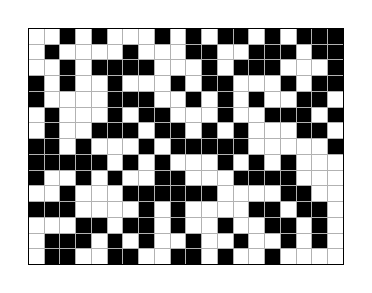
\begin{tikzpicture}[x=2mm,y=2mm]
\fill (2,14) rectangle +(1,1);\fill (4,14) rectangle +(1,1);\fill (8,14) rectangle +(1,1);\fill (10,14) rectangle +(1,1);\fill (12,14) rectangle +(1,1);\fill (13,14) rectangle +(1,1);\fill (15,14) rectangle +(1,1);\fill (17,14) rectangle +(1,1);\fill (18,14) rectangle +(1,1);\fill (19,14) rectangle +(1,1);
\fill (1,13) rectangle +(1,1);\fill (6,13) rectangle +(1,1);\fill (10,13) rectangle +(1,1);\fill (11,13) rectangle +(1,1);\fill (14,13) rectangle +(1,1);\fill (15,13) rectangle +(1,1);\fill (16,13) rectangle +(1,1);\fill (18,13) rectangle +(1,1);\fill (19,13) rectangle +(1,1);
\fill (2,12) rectangle +(1,1);\fill (4,12) rectangle +(1,1);\fill (5,12) rectangle +(1,1);\fill (6,12) rectangle +(1,1);\fill (7,12) rectangle +(1,1);\fill (11,12) rectangle +(1,1);\fill (13,12) rectangle +(1,1);\fill (14,12) rectangle +(1,1);\fill (15,12) rectangle +(1,1);\fill (19,12) rectangle +(1,1);
\fill (0,11) rectangle +(1,1);\fill (2,11) rectangle +(1,1);\fill (5,11) rectangle +(1,1);\fill (9,11) rectangle +(1,1);\fill (11,11) rectangle +(1,1);\fill (12,11) rectangle +(1,1);\fill (16,11) rectangle +(1,1);\fill (18,11) rectangle +(1,1);\fill (19,11) rectangle +(1,1);
\fill (0,10) rectangle +(1,1);\fill (5,10) rectangle +(1,1);\fill (6,10) rectangle +(1,1);\fill (7,10) rectangle +(1,1);\fill (10,10) rectangle +(1,1);\fill (12,10) rectangle +(1,1);\fill (14,10) rectangle +(1,1);\fill (17,10) rectangle +(1,1);\fill (18,10) rectangle +(1,1);
\fill (1,9) rectangle +(1,1);\fill (5,9) rectangle +(1,1);\fill (7,9) rectangle +(1,1);\fill (8,9) rectangle +(1,1);\fill (12,9) rectangle +(1,1);\fill (15,9) rectangle +(1,1);\fill (16,9) rectangle +(1,1);\fill (17,9) rectangle +(1,1);\fill (19,9) rectangle +(1,1);
\fill (1,8) rectangle +(1,1);\fill (4,8) rectangle +(1,1);\fill (5,8) rectangle +(1,1);\fill (6,8) rectangle +(1,1);\fill (8,8) rectangle +(1,1);\fill (9,8) rectangle +(1,1);\fill (11,8) rectangle +(1,1);\fill (13,8) rectangle +(1,1);\fill (17,8) rectangle +(1,1);\fill (18,8) rectangle +(1,1);
\fill (0,7) rectangle +(1,1);\fill (1,7) rectangle +(1,1);\fill (3,7) rectangle +(1,1);\fill (7,7) rectangle +(1,1);\fill (9,7) rectangle +(1,1);\fill (10,7) rectangle +(1,1);\fill (11,7) rectangle +(1,1);\fill (12,7) rectangle +(1,1);\fill (13,7) rectangle +(1,1);\fill (19,7) rectangle +(1,1);
\fill (0,6) rectangle +(1,1);\fill (1,6) rectangle +(1,1);\fill (2,6) rectangle +(1,1);\fill (3,6) rectangle +(1,1);\fill (4,6) rectangle +(1,1);\fill (6,6) rectangle +(1,1);\fill (8,6) rectangle +(1,1);\fill (12,6) rectangle +(1,1);\fill (14,6) rectangle +(1,1);\fill (16,6) rectangle +(1,1);
\fill (0,5) rectangle +(1,1);\fill (3,5) rectangle +(1,1);\fill (5,5) rectangle +(1,1);\fill (8,5) rectangle +(1,1);\fill (9,5) rectangle +(1,1);\fill (13,5) rectangle +(1,1);\fill (14,5) rectangle +(1,1);\fill (15,5) rectangle +(1,1);\fill (16,5) rectangle +(1,1);
\fill (2,4) rectangle +(1,1);\fill (6,4) rectangle +(1,1);\fill (7,4) rectangle +(1,1);\fill (8,4) rectangle +(1,1);\fill (9,4) rectangle +(1,1);\fill (10,4) rectangle +(1,1);\fill (11,4) rectangle +(1,1);\fill (16,4) rectangle +(1,1);\fill (17,4) rectangle +(1,1);
\fill (0,3) rectangle +(1,1);\fill (1,3) rectangle +(1,1);\fill (2,3) rectangle +(1,1);\fill (7,3) rectangle +(1,1);\fill (9,3) rectangle +(1,1);\fill (14,3) rectangle +(1,1);\fill (15,3) rectangle +(1,1);\fill (17,3) rectangle +(1,1);\fill (18,3) rectangle +(1,1);
\fill (3,2) rectangle +(1,1);\fill (4,2) rectangle +(1,1);\fill (6,2) rectangle +(1,1);\fill (7,2) rectangle +(1,1);\fill (9,2) rectangle +(1,1);\fill (12,2) rectangle +(1,1);\fill (15,2) rectangle +(1,1);\fill (16,2) rectangle +(1,1);\fill (18,2) rectangle +(1,1);
\fill (1,1) rectangle +(1,1);\fill (2,1) rectangle +(1,1);\fill (3,1) rectangle +(1,1);\fill (5,1) rectangle +(1,1);\fill (7,1) rectangle +(1,1);\fill (10,1) rectangle +(1,1);\fill (13,1) rectangle +(1,1);\fill (16,1) rectangle +(1,1);\fill (18,1) rectangle +(1,1);
\fill (1,0) rectangle +(1,1);\fill (2,0) rectangle +(1,1);\fill (5,0) rectangle +(1,1);\fill (6,0) rectangle +(1,1);\fill (9,0) rectangle +(1,1);\fill (10,0) rectangle +(1,1);\fill (12,0) rectangle +(1,1);\fill (15,0) rectangle +(1,1);
\draw[black!30,line width=0.3pt,step=1] (0,0) grid (20,15);
\draw[line width=0.4pt] (0,0) rectangle (20,15);
\end{tikzpicture}\\[3pt]
{\small (i) $z(15,20;3,3)\ge 139$}
\end{minipage}

\bigskip
\begin{minipage}[b]{0.32\textwidth}\centering
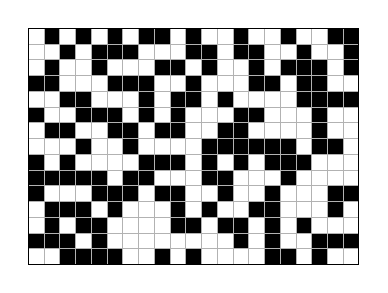
\begin{tikzpicture}[x=2mm,y=2mm]
\fill (1,14) rectangle +(1,1);\fill (3,14) rectangle +(1,1);\fill (5,14) rectangle +(1,1);\fill (7,14) rectangle +(1,1);\fill (8,14) rectangle +(1,1);\fill (10,14) rectangle +(1,1);\fill (13,14) rectangle +(1,1);\fill (16,14) rectangle +(1,1);\fill (19,14) rectangle +(1,1);\fill (20,14) rectangle +(1,1);
\fill (2,13) rectangle +(1,1);\fill (4,13) rectangle +(1,1);\fill (5,13) rectangle +(1,1);\fill (6,13) rectangle +(1,1);\fill (10,13) rectangle +(1,1);\fill (11,13) rectangle +(1,1);\fill (13,13) rectangle +(1,1);\fill (14,13) rectangle +(1,1);\fill (17,13) rectangle +(1,1);\fill (20,13) rectangle +(1,1);
\fill (1,12) rectangle +(1,1);\fill (4,12) rectangle +(1,1);\fill (8,12) rectangle +(1,1);\fill (9,12) rectangle +(1,1);\fill (11,12) rectangle +(1,1);\fill (14,12) rectangle +(1,1);\fill (16,12) rectangle +(1,1);\fill (17,12) rectangle +(1,1);\fill (18,12) rectangle +(1,1);\fill (20,12) rectangle +(1,1);
\fill (0,11) rectangle +(1,1);\fill (1,11) rectangle +(1,1);\fill (5,11) rectangle +(1,1);\fill (6,11) rectangle +(1,1);\fill (7,11) rectangle +(1,1);\fill (10,11) rectangle +(1,1);\fill (14,11) rectangle +(1,1);\fill (15,11) rectangle +(1,1);\fill (17,11) rectangle +(1,1);\fill (18,11) rectangle +(1,1);
\fill (2,10) rectangle +(1,1);\fill (3,10) rectangle +(1,1);\fill (7,10) rectangle +(1,1);\fill (9,10) rectangle +(1,1);\fill (10,10) rectangle +(1,1);\fill (12,10) rectangle +(1,1);\fill (17,10) rectangle +(1,1);\fill (18,10) rectangle +(1,1);\fill (19,10) rectangle +(1,1);\fill (20,10) rectangle +(1,1);
\fill (0,9) rectangle +(1,1);\fill (3,9) rectangle +(1,1);\fill (4,9) rectangle +(1,1);\fill (5,9) rectangle +(1,1);\fill (7,9) rectangle +(1,1);\fill (9,9) rectangle +(1,1);\fill (13,9) rectangle +(1,1);\fill (14,9) rectangle +(1,1);\fill (18,9) rectangle +(1,1);
\fill (1,8) rectangle +(1,1);\fill (2,8) rectangle +(1,1);\fill (5,8) rectangle +(1,1);\fill (6,8) rectangle +(1,1);\fill (8,8) rectangle +(1,1);\fill (9,8) rectangle +(1,1);\fill (12,8) rectangle +(1,1);\fill (13,8) rectangle +(1,1);\fill (18,8) rectangle +(1,1);
\fill (3,7) rectangle +(1,1);\fill (6,7) rectangle +(1,1);\fill (11,7) rectangle +(1,1);\fill (12,7) rectangle +(1,1);\fill (13,7) rectangle +(1,1);\fill (14,7) rectangle +(1,1);\fill (15,7) rectangle +(1,1);\fill (16,7) rectangle +(1,1);\fill (18,7) rectangle +(1,1);\fill (19,7) rectangle +(1,1);
\fill (0,6) rectangle +(1,1);\fill (2,6) rectangle +(1,1);\fill (7,6) rectangle +(1,1);\fill (8,6) rectangle +(1,1);\fill (9,6) rectangle +(1,1);\fill (11,6) rectangle +(1,1);\fill (13,6) rectangle +(1,1);\fill (15,6) rectangle +(1,1);\fill (16,6) rectangle +(1,1);\fill (17,6) rectangle +(1,1);
\fill (0,5) rectangle +(1,1);\fill (1,5) rectangle +(1,1);\fill (2,5) rectangle +(1,1);\fill (3,5) rectangle +(1,1);\fill (4,5) rectangle +(1,1);\fill (6,5) rectangle +(1,1);\fill (7,5) rectangle +(1,1);\fill (11,5) rectangle +(1,1);\fill (12,5) rectangle +(1,1);\fill (16,5) rectangle +(1,1);
\fill (0,4) rectangle +(1,1);\fill (4,4) rectangle +(1,1);\fill (5,4) rectangle +(1,1);\fill (6,4) rectangle +(1,1);\fill (8,4) rectangle +(1,1);\fill (9,4) rectangle +(1,1);\fill (12,4) rectangle +(1,1);\fill (15,4) rectangle +(1,1);\fill (19,4) rectangle +(1,1);\fill (20,4) rectangle +(1,1);
\fill (1,3) rectangle +(1,1);\fill (2,3) rectangle +(1,1);\fill (3,3) rectangle +(1,1);\fill (5,3) rectangle +(1,1);\fill (9,3) rectangle +(1,1);\fill (11,3) rectangle +(1,1);\fill (14,3) rectangle +(1,1);\fill (15,3) rectangle +(1,1);\fill (19,3) rectangle +(1,1);
\fill (1,2) rectangle +(1,1);\fill (3,2) rectangle +(1,1);\fill (4,2) rectangle +(1,1);\fill (9,2) rectangle +(1,1);\fill (10,2) rectangle +(1,1);\fill (12,2) rectangle +(1,1);\fill (13,2) rectangle +(1,1);\fill (15,2) rectangle +(1,1);\fill (17,2) rectangle +(1,1);
\fill (0,1) rectangle +(1,1);\fill (1,1) rectangle +(1,1);\fill (2,1) rectangle +(1,1);\fill (4,1) rectangle +(1,1);\fill (13,1) rectangle +(1,1);\fill (15,1) rectangle +(1,1);\fill (18,1) rectangle +(1,1);\fill (19,1) rectangle +(1,1);\fill (20,1) rectangle +(1,1);
\fill (2,0) rectangle +(1,1);\fill (3,0) rectangle +(1,1);\fill (4,0) rectangle +(1,1);\fill (5,0) rectangle +(1,1);\fill (8,0) rectangle +(1,1);\fill (10,0) rectangle +(1,1);\fill (15,0) rectangle +(1,1);\fill (16,0) rectangle +(1,1);\fill (18,0) rectangle +(1,1);
\draw[black!30,line width=0.3pt,step=1] (0,0) grid (21,15);
\draw[line width=0.4pt] (0,0) rectangle (21,15);
\end{tikzpicture}\\[3pt]
{\small (j) $z(15,21;3,3)\ge 144$}
\end{minipage}\hfill
\begin{minipage}[b]{0.32\textwidth}\centering
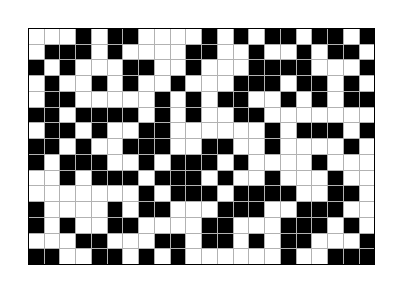
\begin{tikzpicture}[x=2mm,y=2mm]
\fill (3,14) rectangle +(1,1);\fill (5,14) rectangle +(1,1);\fill (6,14) rectangle +(1,1);\fill (11,14) rectangle +(1,1);\fill (13,14) rectangle +(1,1);\fill (15,14) rectangle +(1,1);\fill (16,14) rectangle +(1,1);\fill (18,14) rectangle +(1,1);\fill (19,14) rectangle +(1,1);\fill (21,14) rectangle +(1,1);
\fill (1,13) rectangle +(1,1);\fill (2,13) rectangle +(1,1);\fill (3,13) rectangle +(1,1);\fill (5,13) rectangle +(1,1);\fill (10,13) rectangle +(1,1);\fill (11,13) rectangle +(1,1);\fill (14,13) rectangle +(1,1);\fill (17,13) rectangle +(1,1);\fill (19,13) rectangle +(1,1);\fill (20,13) rectangle +(1,1);
\fill (0,12) rectangle +(1,1);\fill (2,12) rectangle +(1,1);\fill (6,12) rectangle +(1,1);\fill (7,12) rectangle +(1,1);\fill (10,12) rectangle +(1,1);\fill (14,12) rectangle +(1,1);\fill (15,12) rectangle +(1,1);\fill (16,12) rectangle +(1,1);\fill (17,12) rectangle +(1,1);\fill (21,12) rectangle +(1,1);
\fill (1,11) rectangle +(1,1);\fill (4,11) rectangle +(1,1);\fill (6,11) rectangle +(1,1);\fill (9,11) rectangle +(1,1);\fill (13,11) rectangle +(1,1);\fill (14,11) rectangle +(1,1);\fill (15,11) rectangle +(1,1);\fill (17,11) rectangle +(1,1);\fill (18,11) rectangle +(1,1);\fill (20,11) rectangle +(1,1);
\fill (1,10) rectangle +(1,1);\fill (2,10) rectangle +(1,1);\fill (8,10) rectangle +(1,1);\fill (10,10) rectangle +(1,1);\fill (12,10) rectangle +(1,1);\fill (13,10) rectangle +(1,1);\fill (16,10) rectangle +(1,1);\fill (18,10) rectangle +(1,1);\fill (20,10) rectangle +(1,1);\fill (21,10) rectangle +(1,1);
\fill (0,9) rectangle +(1,1);\fill (1,9) rectangle +(1,1);\fill (3,9) rectangle +(1,1);\fill (4,9) rectangle +(1,1);\fill (5,9) rectangle +(1,1);\fill (6,9) rectangle +(1,1);\fill (8,9) rectangle +(1,1);\fill (10,9) rectangle +(1,1);\fill (13,9) rectangle +(1,1);\fill (14,9) rectangle +(1,1);
\fill (1,8) rectangle +(1,1);\fill (2,8) rectangle +(1,1);\fill (4,8) rectangle +(1,1);\fill (7,8) rectangle +(1,1);\fill (8,8) rectangle +(1,1);\fill (15,8) rectangle +(1,1);\fill (17,8) rectangle +(1,1);\fill (18,8) rectangle +(1,1);\fill (19,8) rectangle +(1,1);\fill (21,8) rectangle +(1,1);
\fill (0,7) rectangle +(1,1);\fill (1,7) rectangle +(1,1);\fill (3,7) rectangle +(1,1);\fill (6,7) rectangle +(1,1);\fill (7,7) rectangle +(1,1);\fill (8,7) rectangle +(1,1);\fill (11,7) rectangle +(1,1);\fill (12,7) rectangle +(1,1);\fill (15,7) rectangle +(1,1);\fill (20,7) rectangle +(1,1);
\fill (0,6) rectangle +(1,1);\fill (2,6) rectangle +(1,1);\fill (3,6) rectangle +(1,1);\fill (4,6) rectangle +(1,1);\fill (7,6) rectangle +(1,1);\fill (9,6) rectangle +(1,1);\fill (10,6) rectangle +(1,1);\fill (11,6) rectangle +(1,1);\fill (13,6) rectangle +(1,1);\fill (18,6) rectangle +(1,1);
\fill (2,5) rectangle +(1,1);\fill (4,5) rectangle +(1,1);\fill (5,5) rectangle +(1,1);\fill (6,5) rectangle +(1,1);\fill (8,5) rectangle +(1,1);\fill (9,5) rectangle +(1,1);\fill (10,5) rectangle +(1,1);\fill (12,5) rectangle +(1,1);\fill (15,5) rectangle +(1,1);\fill (19,5) rectangle +(1,1);
\fill (7,4) rectangle +(1,1);\fill (9,4) rectangle +(1,1);\fill (10,4) rectangle +(1,1);\fill (11,4) rectangle +(1,1);\fill (13,4) rectangle +(1,1);\fill (14,4) rectangle +(1,1);\fill (15,4) rectangle +(1,1);\fill (16,4) rectangle +(1,1);\fill (19,4) rectangle +(1,1);\fill (20,4) rectangle +(1,1);
\fill (0,3) rectangle +(1,1);\fill (5,3) rectangle +(1,1);\fill (7,3) rectangle +(1,1);\fill (8,3) rectangle +(1,1);\fill (12,3) rectangle +(1,1);\fill (13,3) rectangle +(1,1);\fill (14,3) rectangle +(1,1);\fill (17,3) rectangle +(1,1);\fill (18,3) rectangle +(1,1);\fill (19,3) rectangle +(1,1);
\fill (0,2) rectangle +(1,1);\fill (2,2) rectangle +(1,1);\fill (5,2) rectangle +(1,1);\fill (6,2) rectangle +(1,1);\fill (11,2) rectangle +(1,1);\fill (12,2) rectangle +(1,1);\fill (16,2) rectangle +(1,1);\fill (17,2) rectangle +(1,1);\fill (18,2) rectangle +(1,1);\fill (20,2) rectangle +(1,1);
\fill (3,1) rectangle +(1,1);\fill (4,1) rectangle +(1,1);\fill (8,1) rectangle +(1,1);\fill (9,1) rectangle +(1,1);\fill (11,1) rectangle +(1,1);\fill (12,1) rectangle +(1,1);\fill (14,1) rectangle +(1,1);\fill (16,1) rectangle +(1,1);\fill (17,1) rectangle +(1,1);\fill (21,1) rectangle +(1,1);
\fill (0,0) rectangle +(1,1);\fill (1,0) rectangle +(1,1);\fill (4,0) rectangle +(1,1);\fill (5,0) rectangle +(1,1);\fill (7,0) rectangle +(1,1);\fill (9,0) rectangle +(1,1);\fill (16,0) rectangle +(1,1);\fill (19,0) rectangle +(1,1);\fill (20,0) rectangle +(1,1);\fill (21,0) rectangle +(1,1);
\draw[black!30,line width=0.3pt,step=1] (0,0) grid (22,15);
\draw[line width=0.4pt] (0,0) rectangle (22,15);
\end{tikzpicture}\\[3pt]
{\small (k) $z(15,22;3,3)\ge 150$}
\end{minipage}\hfill
\begin{minipage}[b]{0.32\textwidth}\centering
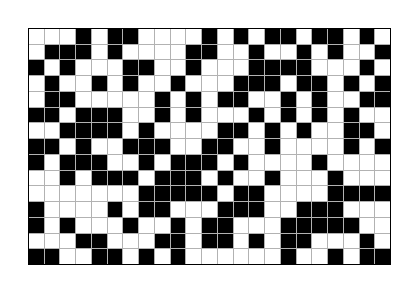
\begin{tikzpicture}[x=2mm,y=2mm]
\fill (3,14) rectangle +(1,1);\fill (5,14) rectangle +(1,1);\fill (6,14) rectangle +(1,1);\fill (11,14) rectangle +(1,1);\fill (13,14) rectangle +(1,1);\fill (15,14) rectangle +(1,1);\fill (16,14) rectangle +(1,1);\fill (18,14) rectangle +(1,1);\fill (19,14) rectangle +(1,1);\fill (21,14) rectangle +(1,1);
\fill (1,13) rectangle +(1,1);\fill (2,13) rectangle +(1,1);\fill (3,13) rectangle +(1,1);\fill (5,13) rectangle +(1,1);\fill (10,13) rectangle +(1,1);\fill (11,13) rectangle +(1,1);\fill (14,13) rectangle +(1,1);\fill (17,13) rectangle +(1,1);\fill (19,13) rectangle +(1,1);\fill (22,13) rectangle +(1,1);
\fill (0,12) rectangle +(1,1);\fill (2,12) rectangle +(1,1);\fill (6,12) rectangle +(1,1);\fill (7,12) rectangle +(1,1);\fill (10,12) rectangle +(1,1);\fill (14,12) rectangle +(1,1);\fill (15,12) rectangle +(1,1);\fill (16,12) rectangle +(1,1);\fill (17,12) rectangle +(1,1);\fill (21,12) rectangle +(1,1);
\fill (1,11) rectangle +(1,1);\fill (4,11) rectangle +(1,1);\fill (6,11) rectangle +(1,1);\fill (9,11) rectangle +(1,1);\fill (13,11) rectangle +(1,1);\fill (14,11) rectangle +(1,1);\fill (15,11) rectangle +(1,1);\fill (17,11) rectangle +(1,1);\fill (18,11) rectangle +(1,1);\fill (20,11) rectangle +(1,1);\fill (22,11) rectangle +(1,1);
\fill (1,10) rectangle +(1,1);\fill (2,10) rectangle +(1,1);\fill (8,10) rectangle +(1,1);\fill (10,10) rectangle +(1,1);\fill (12,10) rectangle +(1,1);\fill (13,10) rectangle +(1,1);\fill (16,10) rectangle +(1,1);\fill (18,10) rectangle +(1,1);\fill (21,10) rectangle +(1,1);\fill (22,10) rectangle +(1,1);
\fill (0,9) rectangle +(1,1);\fill (1,9) rectangle +(1,1);\fill (3,9) rectangle +(1,1);\fill (4,9) rectangle +(1,1);\fill (5,9) rectangle +(1,1);\fill (8,9) rectangle +(1,1);\fill (10,9) rectangle +(1,1);\fill (14,9) rectangle +(1,1);\fill (16,9) rectangle +(1,1);\fill (18,9) rectangle +(1,1);\fill (20,9) rectangle +(1,1);
\fill (2,8) rectangle +(1,1);\fill (3,8) rectangle +(1,1);\fill (4,8) rectangle +(1,1);\fill (5,8) rectangle +(1,1);\fill (7,8) rectangle +(1,1);\fill (12,8) rectangle +(1,1);\fill (13,8) rectangle +(1,1);\fill (15,8) rectangle +(1,1);\fill (17,8) rectangle +(1,1);\fill (20,8) rectangle +(1,1);\fill (21,8) rectangle +(1,1);
\fill (0,7) rectangle +(1,1);\fill (1,7) rectangle +(1,1);\fill (3,7) rectangle +(1,1);\fill (6,7) rectangle +(1,1);\fill (7,7) rectangle +(1,1);\fill (8,7) rectangle +(1,1);\fill (11,7) rectangle +(1,1);\fill (12,7) rectangle +(1,1);\fill (15,7) rectangle +(1,1);\fill (20,7) rectangle +(1,1);\fill (22,7) rectangle +(1,1);
\fill (0,6) rectangle +(1,1);\fill (2,6) rectangle +(1,1);\fill (3,6) rectangle +(1,1);\fill (4,6) rectangle +(1,1);\fill (7,6) rectangle +(1,1);\fill (9,6) rectangle +(1,1);\fill (10,6) rectangle +(1,1);\fill (11,6) rectangle +(1,1);\fill (13,6) rectangle +(1,1);\fill (18,6) rectangle +(1,1);
\fill (2,5) rectangle +(1,1);\fill (4,5) rectangle +(1,1);\fill (5,5) rectangle +(1,1);\fill (6,5) rectangle +(1,1);\fill (8,5) rectangle +(1,1);\fill (9,5) rectangle +(1,1);\fill (10,5) rectangle +(1,1);\fill (12,5) rectangle +(1,1);\fill (15,5) rectangle +(1,1);\fill (19,5) rectangle +(1,1);
\fill (7,4) rectangle +(1,1);\fill (8,4) rectangle +(1,1);\fill (9,4) rectangle +(1,1);\fill (10,4) rectangle +(1,1);\fill (11,4) rectangle +(1,1);\fill (13,4) rectangle +(1,1);\fill (14,4) rectangle +(1,1);\fill (19,4) rectangle +(1,1);\fill (20,4) rectangle +(1,1);\fill (21,4) rectangle +(1,1);\fill (22,4) rectangle +(1,1);
\fill (0,3) rectangle +(1,1);\fill (5,3) rectangle +(1,1);\fill (7,3) rectangle +(1,1);\fill (8,3) rectangle +(1,1);\fill (12,3) rectangle +(1,1);\fill (13,3) rectangle +(1,1);\fill (14,3) rectangle +(1,1);\fill (17,3) rectangle +(1,1);\fill (18,3) rectangle +(1,1);\fill (19,3) rectangle +(1,1);
\fill (0,2) rectangle +(1,1);\fill (2,2) rectangle +(1,1);\fill (6,2) rectangle +(1,1);\fill (9,2) rectangle +(1,1);\fill (11,2) rectangle +(1,1);\fill (12,2) rectangle +(1,1);\fill (16,2) rectangle +(1,1);\fill (17,2) rectangle +(1,1);\fill (18,2) rectangle +(1,1);\fill (19,2) rectangle +(1,1);\fill (20,2) rectangle +(1,1);
\fill (3,1) rectangle +(1,1);\fill (4,1) rectangle +(1,1);\fill (8,1) rectangle +(1,1);\fill (9,1) rectangle +(1,1);\fill (11,1) rectangle +(1,1);\fill (12,1) rectangle +(1,1);\fill (14,1) rectangle +(1,1);\fill (16,1) rectangle +(1,1);\fill (17,1) rectangle +(1,1);\fill (21,1) rectangle +(1,1);
\fill (0,0) rectangle +(1,1);\fill (1,0) rectangle +(1,1);\fill (4,0) rectangle +(1,1);\fill (5,0) rectangle +(1,1);\fill (7,0) rectangle +(1,1);\fill (9,0) rectangle +(1,1);\fill (16,0) rectangle +(1,1);\fill (19,0) rectangle +(1,1);\fill (21,0) rectangle +(1,1);\fill (22,0) rectangle +(1,1);
\draw[black!30,line width=0.3pt,step=1] (0,0) grid (23,15);
\draw[line width=0.4pt] (0,0) rectangle (23,15);
\end{tikzpicture}\\[3pt]
{\small (l) $z(15,23;3,3)\ge 156$}
\end{minipage}

\bigskip
\begin{minipage}[b]{0.32\textwidth}\centering
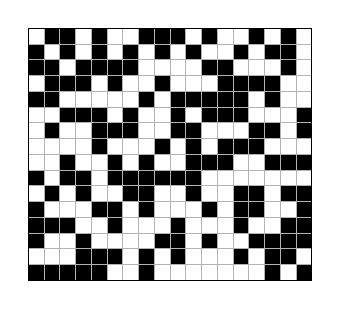
\begin{tikzpicture}[x=2mm,y=2mm]
\fill (1,15) rectangle +(1,1);\fill (2,15) rectangle +(1,1);\fill (4,15) rectangle +(1,1);\fill (7,15) rectangle +(1,1);\fill (8,15) rectangle +(1,1);\fill (9,15) rectangle +(1,1);\fill (11,15) rectangle +(1,1);\fill (14,15) rectangle +(1,1);\fill (16,15) rectangle +(1,1);
\fill (0,14) rectangle +(1,1);\fill (2,14) rectangle +(1,1);\fill (4,14) rectangle +(1,1);\fill (6,14) rectangle +(1,1);\fill (8,14) rectangle +(1,1);\fill (10,14) rectangle +(1,1);\fill (13,14) rectangle +(1,1);\fill (15,14) rectangle +(1,1);\fill (16,14) rectangle +(1,1);
\fill (0,13) rectangle +(1,1);\fill (1,13) rectangle +(1,1);\fill (3,13) rectangle +(1,1);\fill (4,13) rectangle +(1,1);\fill (5,13) rectangle +(1,1);\fill (6,13) rectangle +(1,1);\fill (11,13) rectangle +(1,1);\fill (12,13) rectangle +(1,1);\fill (16,13) rectangle +(1,1);
\fill (1,12) rectangle +(1,1);\fill (2,12) rectangle +(1,1);\fill (3,12) rectangle +(1,1);\fill (5,12) rectangle +(1,1);\fill (8,12) rectangle +(1,1);\fill (12,12) rectangle +(1,1);\fill (13,12) rectangle +(1,1);\fill (14,12) rectangle +(1,1);\fill (15,12) rectangle +(1,1);
\fill (0,11) rectangle +(1,1);\fill (1,11) rectangle +(1,1);\fill (7,11) rectangle +(1,1);\fill (9,11) rectangle +(1,1);\fill (10,11) rectangle +(1,1);\fill (11,11) rectangle +(1,1);\fill (12,11) rectangle +(1,1);\fill (13,11) rectangle +(1,1);\fill (15,11) rectangle +(1,1);
\fill (2,10) rectangle +(1,1);\fill (3,10) rectangle +(1,1);\fill (4,10) rectangle +(1,1);\fill (6,10) rectangle +(1,1);\fill (9,10) rectangle +(1,1);\fill (11,10) rectangle +(1,1);\fill (12,10) rectangle +(1,1);\fill (13,10) rectangle +(1,1);\fill (17,10) rectangle +(1,1);
\fill (1,9) rectangle +(1,1);\fill (4,9) rectangle +(1,1);\fill (5,9) rectangle +(1,1);\fill (6,9) rectangle +(1,1);\fill (9,9) rectangle +(1,1);\fill (10,9) rectangle +(1,1);\fill (14,9) rectangle +(1,1);\fill (15,9) rectangle +(1,1);\fill (17,9) rectangle +(1,1);
\fill (4,8) rectangle +(1,1);\fill (8,8) rectangle +(1,1);\fill (10,8) rectangle +(1,1);\fill (12,8) rectangle +(1,1);\fill (13,8) rectangle +(1,1);\fill (14,8) rectangle +(1,1);
\fill (2,7) rectangle +(1,1);\fill (5,7) rectangle +(1,1);\fill (7,7) rectangle +(1,1);\fill (10,7) rectangle +(1,1);\fill (11,7) rectangle +(1,1);\fill (12,7) rectangle +(1,1);\fill (15,7) rectangle +(1,1);\fill (16,7) rectangle +(1,1);\fill (17,7) rectangle +(1,1);
\fill (0,6) rectangle +(1,1);\fill (2,6) rectangle +(1,1);\fill (3,6) rectangle +(1,1);\fill (5,6) rectangle +(1,1);\fill (6,6) rectangle +(1,1);\fill (7,6) rectangle +(1,1);\fill (8,6) rectangle +(1,1);\fill (9,6) rectangle +(1,1);\fill (10,6) rectangle +(1,1);
\fill (1,5) rectangle +(1,1);\fill (3,5) rectangle +(1,1);\fill (6,5) rectangle +(1,1);\fill (7,5) rectangle +(1,1);\fill (10,5) rectangle +(1,1);\fill (13,5) rectangle +(1,1);\fill (14,5) rectangle +(1,1);\fill (16,5) rectangle +(1,1);\fill (17,5) rectangle +(1,1);
\fill (0,4) rectangle +(1,1);\fill (4,4) rectangle +(1,1);\fill (5,4) rectangle +(1,1);\fill (7,4) rectangle +(1,1);\fill (11,4) rectangle +(1,1);\fill (13,4) rectangle +(1,1);\fill (14,4) rectangle +(1,1);\fill (17,4) rectangle +(1,1);
\fill (0,3) rectangle +(1,1);\fill (1,3) rectangle +(1,1);\fill (2,3) rectangle +(1,1);\fill (5,3) rectangle +(1,1);\fill (9,3) rectangle +(1,1);\fill (13,3) rectangle +(1,1);\fill (16,3) rectangle +(1,1);\fill (17,3) rectangle +(1,1);
\fill (0,2) rectangle +(1,1);\fill (3,2) rectangle +(1,1);\fill (8,2) rectangle +(1,1);\fill (9,2) rectangle +(1,1);\fill (11,2) rectangle +(1,1);\fill (14,2) rectangle +(1,1);\fill (15,2) rectangle +(1,1);\fill (16,2) rectangle +(1,1);\fill (17,2) rectangle +(1,1);
\fill (3,1) rectangle +(1,1);\fill (4,1) rectangle +(1,1);\fill (5,1) rectangle +(1,1);\fill (7,1) rectangle +(1,1);\fill (9,1) rectangle +(1,1);\fill (13,1) rectangle +(1,1);\fill (15,1) rectangle +(1,1);\fill (16,1) rectangle +(1,1);
\fill (0,0) rectangle +(1,1);\fill (1,0) rectangle +(1,1);\fill (2,0) rectangle +(1,1);\fill (3,0) rectangle +(1,1);\fill (4,0) rectangle +(1,1);\fill (7,0) rectangle +(1,1);\fill (15,0) rectangle +(1,1);\fill (17,0) rectangle +(1,1);
\draw[black!30,line width=0.3pt,step=1] (0,0) grid (18,16);
\draw[line width=0.4pt] (0,0) rectangle (18,16);
\end{tikzpicture}\\[3pt]
{\small (m) $z(16,18;3,3)\ge 137$}
\end{minipage}\hfill
\begin{minipage}[b]{0.32\textwidth}\centering
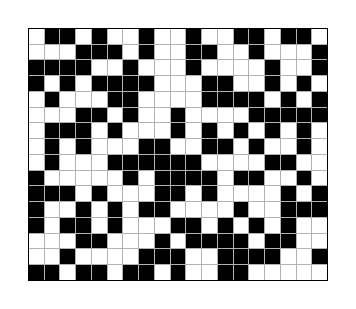
\begin{tikzpicture}[x=2mm,y=2mm]
\fill (1,15) rectangle +(1,1);\fill (2,15) rectangle +(1,1);\fill (4,15) rectangle +(1,1);\fill (7,15) rectangle +(1,1);\fill (10,15) rectangle +(1,1);\fill (13,15) rectangle +(1,1);\fill (14,15) rectangle +(1,1);\fill (16,15) rectangle +(1,1);\fill (17,15) rectangle +(1,1);
\fill (3,14) rectangle +(1,1);\fill (4,14) rectangle +(1,1);\fill (5,14) rectangle +(1,1);\fill (7,14) rectangle +(1,1);\fill (10,14) rectangle +(1,1);\fill (11,14) rectangle +(1,1);\fill (14,14) rectangle +(1,1);\fill (18,14) rectangle +(1,1);
\fill (0,13) rectangle +(1,1);\fill (1,13) rectangle +(1,1);\fill (2,13) rectangle +(1,1);\fill (3,13) rectangle +(1,1);\fill (6,13) rectangle +(1,1);\fill (10,13) rectangle +(1,1);\fill (15,13) rectangle +(1,1);\fill (18,13) rectangle +(1,1);
\fill (0,12) rectangle +(1,1);\fill (2,12) rectangle +(1,1);\fill (4,12) rectangle +(1,1);\fill (5,12) rectangle +(1,1);\fill (6,12) rectangle +(1,1);\fill (7,12) rectangle +(1,1);\fill (11,12) rectangle +(1,1);\fill (12,12) rectangle +(1,1);\fill (15,12) rectangle +(1,1);\fill (17,12) rectangle +(1,1);
\fill (1,11) rectangle +(1,1);\fill (5,11) rectangle +(1,1);\fill (6,11) rectangle +(1,1);\fill (11,11) rectangle +(1,1);\fill (12,11) rectangle +(1,1);\fill (13,11) rectangle +(1,1);\fill (14,11) rectangle +(1,1);\fill (16,11) rectangle +(1,1);\fill (18,11) rectangle +(1,1);
\fill (3,10) rectangle +(1,1);\fill (4,10) rectangle +(1,1);\fill (6,10) rectangle +(1,1);\fill (9,10) rectangle +(1,1);\fill (14,10) rectangle +(1,1);\fill (15,10) rectangle +(1,1);\fill (16,10) rectangle +(1,1);\fill (17,10) rectangle +(1,1);\fill (18,10) rectangle +(1,1);
\fill (1,9) rectangle +(1,1);\fill (2,9) rectangle +(1,1);\fill (3,9) rectangle +(1,1);\fill (5,9) rectangle +(1,1);\fill (9,9) rectangle +(1,1);\fill (11,9) rectangle +(1,1);\fill (13,9) rectangle +(1,1);\fill (15,9) rectangle +(1,1);\fill (17,9) rectangle +(1,1);
\fill (1,8) rectangle +(1,1);\fill (3,8) rectangle +(1,1);\fill (7,8) rectangle +(1,1);\fill (8,8) rectangle +(1,1);\fill (11,8) rectangle +(1,1);\fill (12,8) rectangle +(1,1);\fill (14,8) rectangle +(1,1);\fill (17,8) rectangle +(1,1);
\fill (1,7) rectangle +(1,1);\fill (5,7) rectangle +(1,1);\fill (6,7) rectangle +(1,1);\fill (7,7) rectangle +(1,1);\fill (8,7) rectangle +(1,1);\fill (9,7) rectangle +(1,1);\fill (10,7) rectangle +(1,1);\fill (15,7) rectangle +(1,1);\fill (16,7) rectangle +(1,1);
\fill (0,6) rectangle +(1,1);\fill (6,6) rectangle +(1,1);\fill (8,6) rectangle +(1,1);\fill (9,6) rectangle +(1,1);\fill (10,6) rectangle +(1,1);\fill (11,6) rectangle +(1,1);\fill (13,6) rectangle +(1,1);\fill (14,6) rectangle +(1,1);\fill (17,6) rectangle +(1,1);
\fill (0,5) rectangle +(1,1);\fill (1,5) rectangle +(1,1);\fill (2,5) rectangle +(1,1);\fill (4,5) rectangle +(1,1);\fill (8,5) rectangle +(1,1);\fill (9,5) rectangle +(1,1);\fill (11,5) rectangle +(1,1);\fill (16,5) rectangle +(1,1);\fill (18,5) rectangle +(1,1);
\fill (0,4) rectangle +(1,1);\fill (3,4) rectangle +(1,1);\fill (5,4) rectangle +(1,1);\fill (7,4) rectangle +(1,1);\fill (8,4) rectangle +(1,1);\fill (13,4) rectangle +(1,1);\fill (16,4) rectangle +(1,1);\fill (17,4) rectangle +(1,1);\fill (18,4) rectangle +(1,1);
\fill (0,3) rectangle +(1,1);\fill (2,3) rectangle +(1,1);\fill (3,3) rectangle +(1,1);\fill (5,3) rectangle +(1,1);\fill (9,3) rectangle +(1,1);\fill (10,3) rectangle +(1,1);\fill (12,3) rectangle +(1,1);\fill (14,3) rectangle +(1,1);\fill (16,3) rectangle +(1,1);
\fill (3,2) rectangle +(1,1);\fill (4,2) rectangle +(1,1);\fill (8,2) rectangle +(1,1);\fill (10,2) rectangle +(1,1);\fill (11,2) rectangle +(1,1);\fill (12,2) rectangle +(1,1);\fill (13,2) rectangle +(1,1);\fill (15,2) rectangle +(1,1);\fill (16,2) rectangle +(1,1);
\fill (2,1) rectangle +(1,1);\fill (7,1) rectangle +(1,1);\fill (8,1) rectangle +(1,1);\fill (9,1) rectangle +(1,1);\fill (12,1) rectangle +(1,1);\fill (13,1) rectangle +(1,1);\fill (14,1) rectangle +(1,1);\fill (15,1) rectangle +(1,1);\fill (18,1) rectangle +(1,1);
\fill (0,0) rectangle +(1,1);\fill (1,0) rectangle +(1,1);\fill (3,0) rectangle +(1,1);\fill (4,0) rectangle +(1,1);\fill (6,0) rectangle +(1,1);\fill (7,0) rectangle +(1,1);\fill (9,0) rectangle +(1,1);\fill (12,0) rectangle +(1,1);\fill (13,0) rectangle +(1,1);
\draw[black!30,line width=0.3pt,step=1] (0,0) grid (19,16);
\draw[line width=0.4pt] (0,0) rectangle (19,16);
\end{tikzpicture}\\[3pt]
{\small (n) $z(16,19;3,3)\ge 142$}
\end{minipage}\hfill
\begin{minipage}[b]{0.32\textwidth}\centering
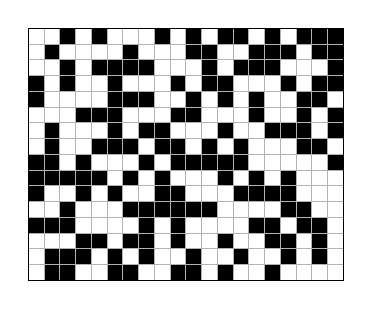
\begin{tikzpicture}[x=2mm,y=2mm]
\fill (2,15) rectangle +(1,1);\fill (4,15) rectangle +(1,1);\fill (8,15) rectangle +(1,1);\fill (10,15) rectangle +(1,1);\fill (12,15) rectangle +(1,1);\fill (13,15) rectangle +(1,1);\fill (15,15) rectangle +(1,1);\fill (17,15) rectangle +(1,1);\fill (18,15) rectangle +(1,1);\fill (19,15) rectangle +(1,1);
\fill (1,14) rectangle +(1,1);\fill (6,14) rectangle +(1,1);\fill (10,14) rectangle +(1,1);\fill (11,14) rectangle +(1,1);\fill (14,14) rectangle +(1,1);\fill (15,14) rectangle +(1,1);\fill (16,14) rectangle +(1,1);\fill (18,14) rectangle +(1,1);\fill (19,14) rectangle +(1,1);
\fill (2,13) rectangle +(1,1);\fill (4,13) rectangle +(1,1);\fill (5,13) rectangle +(1,1);\fill (6,13) rectangle +(1,1);\fill (7,13) rectangle +(1,1);\fill (11,13) rectangle +(1,1);\fill (13,13) rectangle +(1,1);\fill (14,13) rectangle +(1,1);\fill (15,13) rectangle +(1,1);\fill (19,13) rectangle +(1,1);
\fill (0,12) rectangle +(1,1);\fill (2,12) rectangle +(1,1);\fill (5,12) rectangle +(1,1);\fill (9,12) rectangle +(1,1);\fill (11,12) rectangle +(1,1);\fill (12,12) rectangle +(1,1);\fill (16,12) rectangle +(1,1);\fill (18,12) rectangle +(1,1);\fill (19,12) rectangle +(1,1);
\fill (0,11) rectangle +(1,1);\fill (5,11) rectangle +(1,1);\fill (6,11) rectangle +(1,1);\fill (7,11) rectangle +(1,1);\fill (10,11) rectangle +(1,1);\fill (12,11) rectangle +(1,1);\fill (14,11) rectangle +(1,1);\fill (17,11) rectangle +(1,1);\fill (18,11) rectangle +(1,1);
\fill (3,10) rectangle +(1,1);\fill (4,10) rectangle +(1,1);\fill (5,10) rectangle +(1,1);\fill (9,10) rectangle +(1,1);\fill (10,10) rectangle +(1,1);\fill (14,10) rectangle +(1,1);\fill (17,10) rectangle +(1,1);\fill (19,10) rectangle +(1,1);
\fill (1,9) rectangle +(1,1);\fill (5,9) rectangle +(1,1);\fill (7,9) rectangle +(1,1);\fill (8,9) rectangle +(1,1);\fill (12,9) rectangle +(1,1);\fill (15,9) rectangle +(1,1);\fill (16,9) rectangle +(1,1);\fill (17,9) rectangle +(1,1);\fill (19,9) rectangle +(1,1);
\fill (1,8) rectangle +(1,1);\fill (4,8) rectangle +(1,1);\fill (5,8) rectangle +(1,1);\fill (6,8) rectangle +(1,1);\fill (8,8) rectangle +(1,1);\fill (9,8) rectangle +(1,1);\fill (11,8) rectangle +(1,1);\fill (13,8) rectangle +(1,1);\fill (17,8) rectangle +(1,1);\fill (18,8) rectangle +(1,1);
\fill (0,7) rectangle +(1,1);\fill (1,7) rectangle +(1,1);\fill (3,7) rectangle +(1,1);\fill (7,7) rectangle +(1,1);\fill (9,7) rectangle +(1,1);\fill (10,7) rectangle +(1,1);\fill (11,7) rectangle +(1,1);\fill (12,7) rectangle +(1,1);\fill (13,7) rectangle +(1,1);\fill (19,7) rectangle +(1,1);
\fill (0,6) rectangle +(1,1);\fill (1,6) rectangle +(1,1);\fill (2,6) rectangle +(1,1);\fill (3,6) rectangle +(1,1);\fill (4,6) rectangle +(1,1);\fill (6,6) rectangle +(1,1);\fill (8,6) rectangle +(1,1);\fill (12,6) rectangle +(1,1);\fill (14,6) rectangle +(1,1);\fill (16,6) rectangle +(1,1);
\fill (0,5) rectangle +(1,1);\fill (3,5) rectangle +(1,1);\fill (5,5) rectangle +(1,1);\fill (8,5) rectangle +(1,1);\fill (9,5) rectangle +(1,1);\fill (13,5) rectangle +(1,1);\fill (14,5) rectangle +(1,1);\fill (15,5) rectangle +(1,1);\fill (16,5) rectangle +(1,1);
\fill (2,4) rectangle +(1,1);\fill (6,4) rectangle +(1,1);\fill (7,4) rectangle +(1,1);\fill (8,4) rectangle +(1,1);\fill (9,4) rectangle +(1,1);\fill (10,4) rectangle +(1,1);\fill (11,4) rectangle +(1,1);\fill (16,4) rectangle +(1,1);\fill (17,4) rectangle +(1,1);
\fill (0,3) rectangle +(1,1);\fill (1,3) rectangle +(1,1);\fill (2,3) rectangle +(1,1);\fill (7,3) rectangle +(1,1);\fill (9,3) rectangle +(1,1);\fill (14,3) rectangle +(1,1);\fill (15,3) rectangle +(1,1);\fill (17,3) rectangle +(1,1);\fill (18,3) rectangle +(1,1);
\fill (3,2) rectangle +(1,1);\fill (4,2) rectangle +(1,1);\fill (6,2) rectangle +(1,1);\fill (7,2) rectangle +(1,1);\fill (9,2) rectangle +(1,1);\fill (12,2) rectangle +(1,1);\fill (15,2) rectangle +(1,1);\fill (16,2) rectangle +(1,1);\fill (18,2) rectangle +(1,1);
\fill (1,1) rectangle +(1,1);\fill (2,1) rectangle +(1,1);\fill (3,1) rectangle +(1,1);\fill (5,1) rectangle +(1,1);\fill (7,1) rectangle +(1,1);\fill (10,1) rectangle +(1,1);\fill (13,1) rectangle +(1,1);\fill (16,1) rectangle +(1,1);\fill (18,1) rectangle +(1,1);
\fill (1,0) rectangle +(1,1);\fill (2,0) rectangle +(1,1);\fill (5,0) rectangle +(1,1);\fill (6,0) rectangle +(1,1);\fill (9,0) rectangle +(1,1);\fill (10,0) rectangle +(1,1);\fill (12,0) rectangle +(1,1);\fill (15,0) rectangle +(1,1);
\draw[black!30,line width=0.3pt,step=1] (0,0) grid (20,16);
\draw[line width=0.4pt] (0,0) rectangle (20,16);
\end{tikzpicture}\\[3pt]
{\small (o) $z(16,20;3,3)\ge 147$}
\end{minipage}

\bigskip
\begin{minipage}[b]{0.32\textwidth}\centering
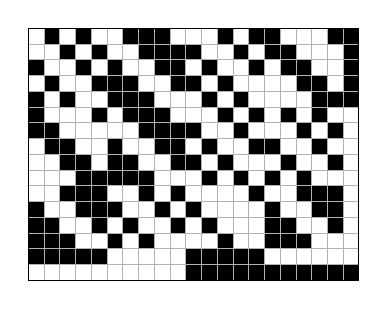
\begin{tikzpicture}[x=2mm,y=2mm]
\fill (1,15) rectangle +(1,1);\fill (3,15) rectangle +(1,1);\fill (6,15) rectangle +(1,1);\fill (7,15) rectangle +(1,1);\fill (8,15) rectangle +(1,1);\fill (12,15) rectangle +(1,1);\fill (14,15) rectangle +(1,1);\fill (15,15) rectangle +(1,1);\fill (19,15) rectangle +(1,1);\fill (20,15) rectangle +(1,1);
\fill (2,14) rectangle +(1,1);\fill (4,14) rectangle +(1,1);\fill (7,14) rectangle +(1,1);\fill (8,14) rectangle +(1,1);\fill (9,14) rectangle +(1,1);\fill (10,14) rectangle +(1,1);\fill (13,14) rectangle +(1,1);\fill (15,14) rectangle +(1,1);\fill (16,14) rectangle +(1,1);\fill (20,14) rectangle +(1,1);
\fill (0,13) rectangle +(1,1);\fill (3,13) rectangle +(1,1);\fill (5,13) rectangle +(1,1);\fill (8,13) rectangle +(1,1);\fill (9,13) rectangle +(1,1);\fill (11,13) rectangle +(1,1);\fill (14,13) rectangle +(1,1);\fill (16,13) rectangle +(1,1);\fill (17,13) rectangle +(1,1);\fill (20,13) rectangle +(1,1);
\fill (1,12) rectangle +(1,1);\fill (4,12) rectangle +(1,1);\fill (5,12) rectangle +(1,1);\fill (6,12) rectangle +(1,1);\fill (9,12) rectangle +(1,1);\fill (10,12) rectangle +(1,1);\fill (12,12) rectangle +(1,1);\fill (17,12) rectangle +(1,1);\fill (18,12) rectangle +(1,1);\fill (20,12) rectangle +(1,1);
\fill (0,11) rectangle +(1,1);\fill (2,11) rectangle +(1,1);\fill (5,11) rectangle +(1,1);\fill (6,11) rectangle +(1,1);\fill (7,11) rectangle +(1,1);\fill (11,11) rectangle +(1,1);\fill (13,11) rectangle +(1,1);\fill (18,11) rectangle +(1,1);\fill (19,11) rectangle +(1,1);\fill (20,11) rectangle +(1,1);
\fill (0,10) rectangle +(1,1);\fill (4,10) rectangle +(1,1);\fill (6,10) rectangle +(1,1);\fill (7,10) rectangle +(1,1);\fill (8,10) rectangle +(1,1);\fill (12,10) rectangle +(1,1);\fill (14,10) rectangle +(1,1);\fill (16,10) rectangle +(1,1);\fill (18,10) rectangle +(1,1);
\fill (0,9) rectangle +(1,1);\fill (1,9) rectangle +(1,1);\fill (7,9) rectangle +(1,1);\fill (8,9) rectangle +(1,1);\fill (9,9) rectangle +(1,1);\fill (10,9) rectangle +(1,1);\fill (13,9) rectangle +(1,1);\fill (17,9) rectangle +(1,1);\fill (19,9) rectangle +(1,1);
\fill (1,8) rectangle +(1,1);\fill (2,8) rectangle +(1,1);\fill (5,8) rectangle +(1,1);\fill (8,8) rectangle +(1,1);\fill (9,8) rectangle +(1,1);\fill (11,8) rectangle +(1,1);\fill (14,8) rectangle +(1,1);\fill (15,8) rectangle +(1,1);\fill (18,8) rectangle +(1,1);
\fill (2,7) rectangle +(1,1);\fill (3,7) rectangle +(1,1);\fill (5,7) rectangle +(1,1);\fill (6,7) rectangle +(1,1);\fill (9,7) rectangle +(1,1);\fill (10,7) rectangle +(1,1);\fill (12,7) rectangle +(1,1);\fill (16,7) rectangle +(1,1);\fill (19,7) rectangle +(1,1);
\fill (3,6) rectangle +(1,1);\fill (4,6) rectangle +(1,1);\fill (5,6) rectangle +(1,1);\fill (6,6) rectangle +(1,1);\fill (7,6) rectangle +(1,1);\fill (11,6) rectangle +(1,1);\fill (13,6) rectangle +(1,1);\fill (15,6) rectangle +(1,1);\fill (17,6) rectangle +(1,1);
\fill (2,5) rectangle +(1,1);\fill (3,5) rectangle +(1,1);\fill (4,5) rectangle +(1,1);\fill (7,5) rectangle +(1,1);\fill (9,5) rectangle +(1,1);\fill (14,5) rectangle +(1,1);\fill (17,5) rectangle +(1,1);\fill (18,5) rectangle +(1,1);\fill (19,5) rectangle +(1,1);
\fill (0,4) rectangle +(1,1);\fill (3,4) rectangle +(1,1);\fill (4,4) rectangle +(1,1);\fill (5,4) rectangle +(1,1);\fill (8,4) rectangle +(1,1);\fill (10,4) rectangle +(1,1);\fill (15,4) rectangle +(1,1);\fill (18,4) rectangle +(1,1);\fill (19,4) rectangle +(1,1);
\fill (0,3) rectangle +(1,1);\fill (1,3) rectangle +(1,1);\fill (4,3) rectangle +(1,1);\fill (6,3) rectangle +(1,1);\fill (9,3) rectangle +(1,1);\fill (11,3) rectangle +(1,1);\fill (15,3) rectangle +(1,1);\fill (16,3) rectangle +(1,1);\fill (19,3) rectangle +(1,1);
\fill (0,2) rectangle +(1,1);\fill (1,2) rectangle +(1,1);\fill (2,2) rectangle +(1,1);\fill (5,2) rectangle +(1,1);\fill (7,2) rectangle +(1,1);\fill (12,2) rectangle +(1,1);\fill (15,2) rectangle +(1,1);\fill (16,2) rectangle +(1,1);\fill (17,2) rectangle +(1,1);
\fill (0,1) rectangle +(1,1);\fill (1,1) rectangle +(1,1);\fill (2,1) rectangle +(1,1);\fill (3,1) rectangle +(1,1);\fill (4,1) rectangle +(1,1);\fill (10,1) rectangle +(1,1);\fill (11,1) rectangle +(1,1);\fill (12,1) rectangle +(1,1);\fill (13,1) rectangle +(1,1);\fill (14,1) rectangle +(1,1);
\fill (10,0) rectangle +(1,1);\fill (11,0) rectangle +(1,1);\fill (12,0) rectangle +(1,1);\fill (13,0) rectangle +(1,1);\fill (14,0) rectangle +(1,1);\fill (15,0) rectangle +(1,1);\fill (16,0) rectangle +(1,1);\fill (17,0) rectangle +(1,1);\fill (18,0) rectangle +(1,1);\fill (19,0) rectangle +(1,1);\fill (20,0) rectangle +(1,1);
\draw[black!30,line width=0.3pt,step=1] (0,0) grid (21,16);
\draw[line width=0.4pt] (0,0) rectangle (21,16);
\end{tikzpicture}\\[3pt]
{\small (p) $z(16,21;3,3)\ge 152$}
\end{minipage}\hfill
\begin{minipage}[b]{0.32\textwidth}\centering
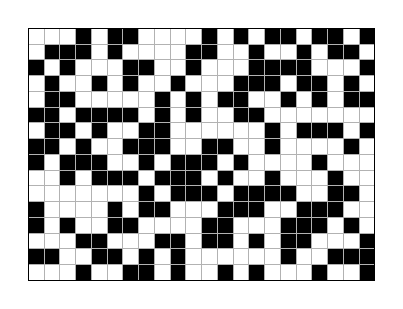
\begin{tikzpicture}[x=2mm,y=2mm]
\fill (3,15) rectangle +(1,1);\fill (5,15) rectangle +(1,1);\fill (6,15) rectangle +(1,1);\fill (11,15) rectangle +(1,1);\fill (13,15) rectangle +(1,1);\fill (15,15) rectangle +(1,1);\fill (16,15) rectangle +(1,1);\fill (18,15) rectangle +(1,1);\fill (19,15) rectangle +(1,1);\fill (21,15) rectangle +(1,1);
\fill (1,14) rectangle +(1,1);\fill (2,14) rectangle +(1,1);\fill (3,14) rectangle +(1,1);\fill (5,14) rectangle +(1,1);\fill (10,14) rectangle +(1,1);\fill (11,14) rectangle +(1,1);\fill (14,14) rectangle +(1,1);\fill (17,14) rectangle +(1,1);\fill (19,14) rectangle +(1,1);\fill (20,14) rectangle +(1,1);
\fill (0,13) rectangle +(1,1);\fill (2,13) rectangle +(1,1);\fill (6,13) rectangle +(1,1);\fill (7,13) rectangle +(1,1);\fill (10,13) rectangle +(1,1);\fill (14,13) rectangle +(1,1);\fill (15,13) rectangle +(1,1);\fill (16,13) rectangle +(1,1);\fill (17,13) rectangle +(1,1);\fill (21,13) rectangle +(1,1);
\fill (1,12) rectangle +(1,1);\fill (4,12) rectangle +(1,1);\fill (6,12) rectangle +(1,1);\fill (9,12) rectangle +(1,1);\fill (13,12) rectangle +(1,1);\fill (14,12) rectangle +(1,1);\fill (15,12) rectangle +(1,1);\fill (17,12) rectangle +(1,1);\fill (18,12) rectangle +(1,1);\fill (20,12) rectangle +(1,1);
\fill (1,11) rectangle +(1,1);\fill (2,11) rectangle +(1,1);\fill (8,11) rectangle +(1,1);\fill (10,11) rectangle +(1,1);\fill (12,11) rectangle +(1,1);\fill (13,11) rectangle +(1,1);\fill (16,11) rectangle +(1,1);\fill (18,11) rectangle +(1,1);\fill (20,11) rectangle +(1,1);\fill (21,11) rectangle +(1,1);
\fill (0,10) rectangle +(1,1);\fill (1,10) rectangle +(1,1);\fill (3,10) rectangle +(1,1);\fill (4,10) rectangle +(1,1);\fill (5,10) rectangle +(1,1);\fill (6,10) rectangle +(1,1);\fill (8,10) rectangle +(1,1);\fill (10,10) rectangle +(1,1);\fill (13,10) rectangle +(1,1);\fill (14,10) rectangle +(1,1);
\fill (1,9) rectangle +(1,1);\fill (2,9) rectangle +(1,1);\fill (4,9) rectangle +(1,1);\fill (7,9) rectangle +(1,1);\fill (8,9) rectangle +(1,1);\fill (15,9) rectangle +(1,1);\fill (17,9) rectangle +(1,1);\fill (18,9) rectangle +(1,1);\fill (19,9) rectangle +(1,1);\fill (21,9) rectangle +(1,1);
\fill (0,8) rectangle +(1,1);\fill (1,8) rectangle +(1,1);\fill (3,8) rectangle +(1,1);\fill (6,8) rectangle +(1,1);\fill (7,8) rectangle +(1,1);\fill (8,8) rectangle +(1,1);\fill (11,8) rectangle +(1,1);\fill (12,8) rectangle +(1,1);\fill (15,8) rectangle +(1,1);\fill (20,8) rectangle +(1,1);
\fill (0,7) rectangle +(1,1);\fill (2,7) rectangle +(1,1);\fill (3,7) rectangle +(1,1);\fill (4,7) rectangle +(1,1);\fill (7,7) rectangle +(1,1);\fill (9,7) rectangle +(1,1);\fill (10,7) rectangle +(1,1);\fill (11,7) rectangle +(1,1);\fill (13,7) rectangle +(1,1);\fill (18,7) rectangle +(1,1);
\fill (2,6) rectangle +(1,1);\fill (4,6) rectangle +(1,1);\fill (5,6) rectangle +(1,1);\fill (6,6) rectangle +(1,1);\fill (8,6) rectangle +(1,1);\fill (9,6) rectangle +(1,1);\fill (10,6) rectangle +(1,1);\fill (12,6) rectangle +(1,1);\fill (15,6) rectangle +(1,1);\fill (19,6) rectangle +(1,1);
\fill (7,5) rectangle +(1,1);\fill (9,5) rectangle +(1,1);\fill (10,5) rectangle +(1,1);\fill (11,5) rectangle +(1,1);\fill (13,5) rectangle +(1,1);\fill (14,5) rectangle +(1,1);\fill (15,5) rectangle +(1,1);\fill (16,5) rectangle +(1,1);\fill (19,5) rectangle +(1,1);\fill (20,5) rectangle +(1,1);
\fill (0,4) rectangle +(1,1);\fill (5,4) rectangle +(1,1);\fill (7,4) rectangle +(1,1);\fill (8,4) rectangle +(1,1);\fill (12,4) rectangle +(1,1);\fill (13,4) rectangle +(1,1);\fill (14,4) rectangle +(1,1);\fill (17,4) rectangle +(1,1);\fill (18,4) rectangle +(1,1);\fill (19,4) rectangle +(1,1);
\fill (0,3) rectangle +(1,1);\fill (2,3) rectangle +(1,1);\fill (5,3) rectangle +(1,1);\fill (6,3) rectangle +(1,1);\fill (11,3) rectangle +(1,1);\fill (12,3) rectangle +(1,1);\fill (16,3) rectangle +(1,1);\fill (17,3) rectangle +(1,1);\fill (18,3) rectangle +(1,1);\fill (20,3) rectangle +(1,1);
\fill (3,2) rectangle +(1,1);\fill (4,2) rectangle +(1,1);\fill (8,2) rectangle +(1,1);\fill (9,2) rectangle +(1,1);\fill (11,2) rectangle +(1,1);\fill (12,2) rectangle +(1,1);\fill (14,2) rectangle +(1,1);\fill (16,2) rectangle +(1,1);\fill (17,2) rectangle +(1,1);\fill (21,2) rectangle +(1,1);
\fill (0,1) rectangle +(1,1);\fill (1,1) rectangle +(1,1);\fill (4,1) rectangle +(1,1);\fill (5,1) rectangle +(1,1);\fill (7,1) rectangle +(1,1);\fill (9,1) rectangle +(1,1);\fill (16,1) rectangle +(1,1);\fill (19,1) rectangle +(1,1);\fill (20,1) rectangle +(1,1);\fill (21,1) rectangle +(1,1);
\fill (3,0) rectangle +(1,1);\fill (6,0) rectangle +(1,1);\fill (7,0) rectangle +(1,1);\fill (9,0) rectangle +(1,1);\fill (12,0) rectangle +(1,1);\fill (14,0) rectangle +(1,1);\fill (18,0) rectangle +(1,1);\fill (21,0) rectangle +(1,1);
\draw[black!30,line width=0.3pt,step=1] (0,0) grid (22,16);
\draw[line width=0.4pt] (0,0) rectangle (22,16);
\end{tikzpicture}\\[3pt]
{\small (q) $z(16,22;3,3)\ge 158$}
\end{minipage}\hfill
\begin{minipage}[b]{0.32\textwidth}\centering
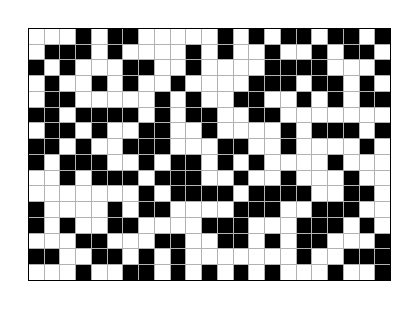
\begin{tikzpicture}[x=2mm,y=2mm]
\fill (3,15) rectangle +(1,1);\fill (5,15) rectangle +(1,1);\fill (6,15) rectangle +(1,1);\fill (12,15) rectangle +(1,1);\fill (14,15) rectangle +(1,1);\fill (16,15) rectangle +(1,1);\fill (17,15) rectangle +(1,1);\fill (19,15) rectangle +(1,1);\fill (20,15) rectangle +(1,1);\fill (22,15) rectangle +(1,1);
\fill (1,14) rectangle +(1,1);\fill (2,14) rectangle +(1,1);\fill (3,14) rectangle +(1,1);\fill (5,14) rectangle +(1,1);\fill (10,14) rectangle +(1,1);\fill (12,14) rectangle +(1,1);\fill (15,14) rectangle +(1,1);\fill (18,14) rectangle +(1,1);\fill (20,14) rectangle +(1,1);\fill (21,14) rectangle +(1,1);
\fill (0,13) rectangle +(1,1);\fill (2,13) rectangle +(1,1);\fill (6,13) rectangle +(1,1);\fill (7,13) rectangle +(1,1);\fill (10,13) rectangle +(1,1);\fill (15,13) rectangle +(1,1);\fill (16,13) rectangle +(1,1);\fill (17,13) rectangle +(1,1);\fill (18,13) rectangle +(1,1);\fill (22,13) rectangle +(1,1);
\fill (1,12) rectangle +(1,1);\fill (4,12) rectangle +(1,1);\fill (6,12) rectangle +(1,1);\fill (9,12) rectangle +(1,1);\fill (14,12) rectangle +(1,1);\fill (15,12) rectangle +(1,1);\fill (16,12) rectangle +(1,1);\fill (18,12) rectangle +(1,1);\fill (19,12) rectangle +(1,1);\fill (21,12) rectangle +(1,1);
\fill (1,11) rectangle +(1,1);\fill (2,11) rectangle +(1,1);\fill (8,11) rectangle +(1,1);\fill (10,11) rectangle +(1,1);\fill (13,11) rectangle +(1,1);\fill (14,11) rectangle +(1,1);\fill (17,11) rectangle +(1,1);\fill (19,11) rectangle +(1,1);\fill (21,11) rectangle +(1,1);\fill (22,11) rectangle +(1,1);
\fill (0,10) rectangle +(1,1);\fill (1,10) rectangle +(1,1);\fill (3,10) rectangle +(1,1);\fill (4,10) rectangle +(1,1);\fill (5,10) rectangle +(1,1);\fill (6,10) rectangle +(1,1);\fill (8,10) rectangle +(1,1);\fill (10,10) rectangle +(1,1);\fill (11,10) rectangle +(1,1);\fill (14,10) rectangle +(1,1);\fill (15,10) rectangle +(1,1);
\fill (1,9) rectangle +(1,1);\fill (2,9) rectangle +(1,1);\fill (4,9) rectangle +(1,1);\fill (7,9) rectangle +(1,1);\fill (8,9) rectangle +(1,1);\fill (11,9) rectangle +(1,1);\fill (16,9) rectangle +(1,1);\fill (18,9) rectangle +(1,1);\fill (19,9) rectangle +(1,1);\fill (20,9) rectangle +(1,1);\fill (22,9) rectangle +(1,1);
\fill (0,8) rectangle +(1,1);\fill (1,8) rectangle +(1,1);\fill (3,8) rectangle +(1,1);\fill (6,8) rectangle +(1,1);\fill (7,8) rectangle +(1,1);\fill (8,8) rectangle +(1,1);\fill (12,8) rectangle +(1,1);\fill (13,8) rectangle +(1,1);\fill (16,8) rectangle +(1,1);\fill (21,8) rectangle +(1,1);
\fill (0,7) rectangle +(1,1);\fill (2,7) rectangle +(1,1);\fill (3,7) rectangle +(1,1);\fill (4,7) rectangle +(1,1);\fill (7,7) rectangle +(1,1);\fill (9,7) rectangle +(1,1);\fill (10,7) rectangle +(1,1);\fill (12,7) rectangle +(1,1);\fill (14,7) rectangle +(1,1);\fill (19,7) rectangle +(1,1);
\fill (2,6) rectangle +(1,1);\fill (4,6) rectangle +(1,1);\fill (5,6) rectangle +(1,1);\fill (6,6) rectangle +(1,1);\fill (8,6) rectangle +(1,1);\fill (9,6) rectangle +(1,1);\fill (10,6) rectangle +(1,1);\fill (13,6) rectangle +(1,1);\fill (16,6) rectangle +(1,1);\fill (20,6) rectangle +(1,1);
\fill (7,5) rectangle +(1,1);\fill (9,5) rectangle +(1,1);\fill (10,5) rectangle +(1,1);\fill (11,5) rectangle +(1,1);\fill (12,5) rectangle +(1,1);\fill (14,5) rectangle +(1,1);\fill (15,5) rectangle +(1,1);\fill (16,5) rectangle +(1,1);\fill (17,5) rectangle +(1,1);\fill (20,5) rectangle +(1,1);\fill (21,5) rectangle +(1,1);
\fill (0,4) rectangle +(1,1);\fill (5,4) rectangle +(1,1);\fill (7,4) rectangle +(1,1);\fill (8,4) rectangle +(1,1);\fill (13,4) rectangle +(1,1);\fill (14,4) rectangle +(1,1);\fill (15,4) rectangle +(1,1);\fill (18,4) rectangle +(1,1);\fill (19,4) rectangle +(1,1);\fill (20,4) rectangle +(1,1);
\fill (0,3) rectangle +(1,1);\fill (2,3) rectangle +(1,1);\fill (5,3) rectangle +(1,1);\fill (6,3) rectangle +(1,1);\fill (11,3) rectangle +(1,1);\fill (12,3) rectangle +(1,1);\fill (13,3) rectangle +(1,1);\fill (17,3) rectangle +(1,1);\fill (18,3) rectangle +(1,1);\fill (19,3) rectangle +(1,1);\fill (21,3) rectangle +(1,1);
\fill (3,2) rectangle +(1,1);\fill (4,2) rectangle +(1,1);\fill (8,2) rectangle +(1,1);\fill (9,2) rectangle +(1,1);\fill (12,2) rectangle +(1,1);\fill (13,2) rectangle +(1,1);\fill (15,2) rectangle +(1,1);\fill (17,2) rectangle +(1,1);\fill (18,2) rectangle +(1,1);\fill (22,2) rectangle +(1,1);
\fill (0,1) rectangle +(1,1);\fill (1,1) rectangle +(1,1);\fill (4,1) rectangle +(1,1);\fill (5,1) rectangle +(1,1);\fill (7,1) rectangle +(1,1);\fill (9,1) rectangle +(1,1);\fill (17,1) rectangle +(1,1);\fill (20,1) rectangle +(1,1);\fill (21,1) rectangle +(1,1);\fill (22,1) rectangle +(1,1);
\fill (3,0) rectangle +(1,1);\fill (6,0) rectangle +(1,1);\fill (7,0) rectangle +(1,1);\fill (9,0) rectangle +(1,1);\fill (11,0) rectangle +(1,1);\fill (13,0) rectangle +(1,1);\fill (15,0) rectangle +(1,1);\fill (19,0) rectangle +(1,1);\fill (22,0) rectangle +(1,1);
\draw[black!30,line width=0.3pt,step=1] (0,0) grid (23,16);
\draw[line width=0.4pt] (0,0) rectangle (23,16);
\end{tikzpicture}\\[3pt]
{\small (r) $z(16,23;3,3)\ge 163$}
\end{minipage}

\bigskip


\end{document}
